\documentclass[conference]{IEEEtran}
\usepackage[T1]{fontenc}
\usepackage{newtxtext}
\usepackage{newtxmath}
\usepackage{amsmath}
\usepackage{booktabs}
\usepackage{array}
\usepackage{siunitx}
\usepackage{graphicx}
\usepackage[caption=false,font=footnotesize]{subfig}
\usepackage{cite}
\usepackage[hyphens]{url}
\usepackage{xcolor}
\usepackage{tikz}
\usetikzlibrary{arrows.meta,positioning,fit,calc,backgrounds}

% ---------------------------------------------------------------------------
% One place for the system name. The code base calls the project MCTS-Rewrite;
% the experiments in this paper do not run its Monte Carlo tree search
% controller, so the paper uses a name that describes what is evaluated.
\newcommand{\sys}{VeriProbe}
% Numbers: generated from the raw logs by paper/scripts/build_data.py.
% Generated by paper/scripts/build_data.py. Do not edit.
\newcommand{\Tmax}{300}
\newcommand{\ThetaPct}{10}
\newcommand{\UnknownCutoff}{20}
\newcommand{\DevN}{30}
\newcommand{\DevOrigMean}{168.8}
\newcommand{\DevOrigMeanU}{168.8}
\newcommand{\DevOrigCensored}{10}
\newcommand{\DevOrigLive}{0}
\newcommand{\DevRbotMean}{[63.5, 138.2]}
\newcommand{\DevRbotMeanL}{63.5}
\newcommand{\DevRbotMeanU}{138.2}
\newcommand{\DevRbotRewrites}{15}
\newcommand{\DevRbotCensored}{8}
\newcommand{\DevRbotFaster}{7}
\newcommand{\DevRbotSlower}{0}
\newcommand{\DevRbotWithin}{0}
\newcommand{\DevRbotUndet}{8}
\newcommand{\DevRbotSame}{15}
\newcommand{\DevRbotRedL}{62.4}
\newcommand{\DevRbotRedU}{18.2}
\newcommand{\DevRbotOursFaster}{14}
\newcommand{\DevRbotOursSlower}{0}
\newcommand{\DevRbotOursWithin}{0}
\newcommand{\DevRbotOursUndet}{6}
\newcommand{\DevRbotOursSame}{10}
\newcommand{\DevRbotGuardedMean}{[63.5, 121.6]}
\newcommand{\DevQuiteMean}{[99.4, 127.4]}
\newcommand{\DevQuiteMeanL}{99.4}
\newcommand{\DevQuiteMeanU}{127.4}
\newcommand{\DevQuiteRewrites}{12}
\newcommand{\DevQuiteCensored}{3}
\newcommand{\DevQuiteFaster}{9}
\newcommand{\DevQuiteSlower}{0}
\newcommand{\DevQuiteWithin}{0}
\newcommand{\DevQuiteUndet}{3}
\newcommand{\DevQuiteSame}{18}
\newcommand{\DevQuiteRedL}{41.1}
\newcommand{\DevQuiteRedU}{24.5}
\newcommand{\DevQuiteOursFaster}{15}
\newcommand{\DevQuiteOursSlower}{0}
\newcommand{\DevQuiteOursWithin}{2}
\newcommand{\DevQuiteOursUndet}{3}
\newcommand{\DevQuiteOursSame}{10}
\newcommand{\DevQuiteGuardedMean}{[99.4, 127.4]}
\newcommand{\DevOursMean}{62.3}
\newcommand{\DevOursMeanL}{62.3}
\newcommand{\DevOursMeanU}{62.3}
\newcommand{\DevOursRewrites}{22}
\newcommand{\DevOursCensored}{0}
\newcommand{\DevOursFaster}{22}
\newcommand{\DevOursSlower}{0}
\newcommand{\DevOursWithin}{0}
\newcommand{\DevOursUndet}{0}
\newcommand{\DevOursSame}{8}
\newcommand{\DevOursRedL}{63.1}
\newcommand{\DevOursRedU}{63.1}
\newcommand{\DevPool}{260}
\newcommand{\DevAccepted}{211}
\newcommand{\DevRejectedPct}{18.8}
\newcommand{\DevSrcMacro}{8}
\newcommand{\DevSrcRule}{4}
\newcommand{\DevSrcQuite}{4}
\newcommand{\DevSrcHint}{5}
\newcommand{\DevSrcRewriteHint}{1}
\newcommand{\DevSrcFallback}{8}
\newcommand{\DevEvSyntactic}{5}
\newcommand{\DevCandEvSyntactic}{30}
\newcommand{\DevEvStructural}{1}
\newcommand{\DevCandEvStructural}{1}
\newcommand{\DevEvSolver}{0}
\newcommand{\DevCandEvSolver}{0}
\newcommand{\DevEvDifferential}{16}
\newcommand{\DevCandEvDifferential}{180}
\newcommand{\DevDepthTwo}{1}
\newcommand{\TpchHeldN}{97}
\newcommand{\TpchHeldOrigMean}{106.3}
\newcommand{\TpchHeldOrigMeanU}{106.3}
\newcommand{\TpchHeldOrigCensored}{20}
\newcommand{\TpchHeldOrigLive}{95}
\newcommand{\TpchHeldRbotMean}{[89.7, 97.8]}
\newcommand{\TpchHeldRbotMeanL}{89.7}
\newcommand{\TpchHeldRbotMeanU}{97.8}
\newcommand{\TpchHeldRbotRewrites}{6}
\newcommand{\TpchHeldRbotCensored}{3}
\newcommand{\TpchHeldRbotFaster}{3}
\newcommand{\TpchHeldRbotSlower}{0}
\newcommand{\TpchHeldRbotWithin}{0}
\newcommand{\TpchHeldRbotUndet}{3}
\newcommand{\TpchHeldRbotSame}{91}
\newcommand{\TpchHeldRbotRedL}{15.6}
\newcommand{\TpchHeldRbotRedU}{7.9}
\newcommand{\TpchHeldRbotOursFaster}{6}
\newcommand{\TpchHeldRbotOursSlower}{1}
\newcommand{\TpchHeldRbotOursWithin}{0}
\newcommand{\TpchHeldRbotOursUndet}{3}
\newcommand{\TpchHeldRbotOursSame}{87}
\newcommand{\TpchHeldRbotGuardedMean}{[89.7, 97.8]}
\newcommand{\TpchHeldQuiteMean}{[102.9, 131.8]}
\newcommand{\TpchHeldQuiteMeanL}{102.9}
\newcommand{\TpchHeldQuiteMeanU}{131.8}
\newcommand{\TpchHeldQuiteRewrites}{11}
\newcommand{\TpchHeldQuiteCensored}{11}
\newcommand{\TpchHeldQuiteFaster}{0}
\newcommand{\TpchHeldQuiteSlower}{0}
\newcommand{\TpchHeldQuiteWithin}{0}
\newcommand{\TpchHeldQuiteUndet}{11}
\newcommand{\TpchHeldQuiteSame}{86}
\newcommand{\TpchHeldQuiteRedL}{3.1}
\newcommand{\TpchHeldQuiteRedU}{-24.1}
\newcommand{\TpchHeldQuiteOursFaster}{8}
\newcommand{\TpchHeldQuiteOursSlower}{0}
\newcommand{\TpchHeldQuiteOursWithin}{0}
\newcommand{\TpchHeldQuiteOursUndet}{11}
\newcommand{\TpchHeldQuiteOursSame}{78}
\newcommand{\TpchHeldQuiteGuardedMean}{[102.9, 106.3]}
\newcommand{\TpchHeldOursMean}{100.0}
\newcommand{\TpchHeldOursMeanL}{100.0}
\newcommand{\TpchHeldOursMeanU}{100.0}
\newcommand{\TpchHeldOursRewrites}{8}
\newcommand{\TpchHeldOursCensored}{0}
\newcommand{\TpchHeldOursFaster}{8}
\newcommand{\TpchHeldOursSlower}{0}
\newcommand{\TpchHeldOursWithin}{0}
\newcommand{\TpchHeldOursUndet}{0}
\newcommand{\TpchHeldOursSame}{89}
\newcommand{\TpchHeldOursRedL}{5.9}
\newcommand{\TpchHeldOursRedU}{5.9}
\newcommand{\TpchHeldPool}{203}
\newcommand{\TpchHeldAccepted}{65}
\newcommand{\TpchHeldRejectedPct}{68.0}
\newcommand{\TpchHeldSrcMacro}{4}
\newcommand{\TpchHeldSrcRule}{4}
\newcommand{\TpchHeldSrcQuite}{0}
\newcommand{\TpchHeldSrcHint}{0}
\newcommand{\TpchHeldSrcRewriteHint}{0}
\newcommand{\TpchHeldSrcFallback}{89}
\newcommand{\TpchHeldEvSyntactic}{0}
\newcommand{\TpchHeldCandEvSyntactic}{9}
\newcommand{\TpchHeldEvStructural}{0}
\newcommand{\TpchHeldCandEvStructural}{0}
\newcommand{\TpchHeldEvSolver}{0}
\newcommand{\TpchHeldCandEvSolver}{0}
\newcommand{\TpchHeldEvDifferential}{8}
\newcommand{\TpchHeldCandEvDifferential}{56}
\newcommand{\TpchHeldDepthTwo}{0}
\newcommand{\CalciteHeldN}{34}
\newcommand{\CalciteHeldOrigMean}{98.5}
\newcommand{\CalciteHeldOrigMeanU}{98.5}
\newcommand{\CalciteHeldOrigCensored}{10}
\newcommand{\CalciteHeldOrigLive}{34}
\newcommand{\CalciteHeldRbotMean}{[28.2, 52.0]}
\newcommand{\CalciteHeldRbotMeanL}{28.2}
\newcommand{\CalciteHeldRbotMeanU}{52.0}
\newcommand{\CalciteHeldRbotRewrites}{12}
\newcommand{\CalciteHeldRbotCensored}{3}
\newcommand{\CalciteHeldRbotFaster}{9}
\newcommand{\CalciteHeldRbotSlower}{0}
\newcommand{\CalciteHeldRbotWithin}{0}
\newcommand{\CalciteHeldRbotUndet}{3}
\newcommand{\CalciteHeldRbotSame}{22}
\newcommand{\CalciteHeldRbotRedL}{71.4}
\newcommand{\CalciteHeldRbotRedU}{47.2}
\newcommand{\CalciteHeldRbotOursFaster}{8}
\newcommand{\CalciteHeldRbotOursSlower}{0}
\newcommand{\CalciteHeldRbotOursWithin}{1}
\newcommand{\CalciteHeldRbotOursUndet}{3}
\newcommand{\CalciteHeldRbotOursSame}{22}
\newcommand{\CalciteHeldRbotGuardedMean}{[28.2, 43.2]}
\newcommand{\CalciteHeldQuiteMean}{[74.7, 89.7]}
\newcommand{\CalciteHeldQuiteMeanL}{74.7}
\newcommand{\CalciteHeldQuiteMeanU}{89.7}
\newcommand{\CalciteHeldQuiteRewrites}{5}
\newcommand{\CalciteHeldQuiteCensored}{2}
\newcommand{\CalciteHeldQuiteFaster}{2}
\newcommand{\CalciteHeldQuiteSlower}{1}
\newcommand{\CalciteHeldQuiteWithin}{0}
\newcommand{\CalciteHeldQuiteUndet}{2}
\newcommand{\CalciteHeldQuiteSame}{29}
\newcommand{\CalciteHeldQuiteRedL}{24.2}
\newcommand{\CalciteHeldQuiteRedU}{8.9}
\newcommand{\CalciteHeldQuiteOursFaster}{14}
\newcommand{\CalciteHeldQuiteOursSlower}{0}
\newcommand{\CalciteHeldQuiteOursWithin}{1}
\newcommand{\CalciteHeldQuiteOursUndet}{1}
\newcommand{\CalciteHeldQuiteOursSame}{18}
\newcommand{\CalciteHeldQuiteGuardedMean}{[74.5, 89.5]}
\newcommand{\CalciteHeldOursMean}{40.8}
\newcommand{\CalciteHeldOursMeanL}{40.8}
\newcommand{\CalciteHeldOursMeanU}{40.8}
\newcommand{\CalciteHeldOursRewrites}{15}
\newcommand{\CalciteHeldOursCensored}{0}
\newcommand{\CalciteHeldOursFaster}{15}
\newcommand{\CalciteHeldOursSlower}{0}
\newcommand{\CalciteHeldOursWithin}{0}
\newcommand{\CalciteHeldOursUndet}{0}
\newcommand{\CalciteHeldOursSame}{19}
\newcommand{\CalciteHeldOursRedL}{58.6}
\newcommand{\CalciteHeldOursRedU}{58.6}
\newcommand{\CalciteHeldPool}{88}
\newcommand{\CalciteHeldAccepted}{51}
\newcommand{\CalciteHeldRejectedPct}{42.0}
\newcommand{\CalciteHeldSrcMacro}{4}
\newcommand{\CalciteHeldSrcRule}{11}
\newcommand{\CalciteHeldSrcQuite}{0}
\newcommand{\CalciteHeldSrcHint}{0}
\newcommand{\CalciteHeldSrcRewriteHint}{0}
\newcommand{\CalciteHeldSrcFallback}{19}
\newcommand{\CalciteHeldEvSyntactic}{0}
\newcommand{\CalciteHeldCandEvSyntactic}{3}
\newcommand{\CalciteHeldEvStructural}{0}
\newcommand{\CalciteHeldCandEvStructural}{0}
\newcommand{\CalciteHeldEvSolver}{0}
\newcommand{\CalciteHeldCandEvSolver}{0}
\newcommand{\CalciteHeldEvDifferential}{15}
\newcommand{\CalciteHeldCandEvDifferential}{48}
\newcommand{\CalciteHeldDepthTwo}{0}
\newcommand{\ZipfN}{30}
\newcommand{\ZipfOrigMean}{133.9}
\newcommand{\ZipfOrigMeanU}{133.9}
\newcommand{\ZipfOrigCensored}{10}
\newcommand{\ZipfOrigLive}{30}
\newcommand{\ZipfRbotMean}{[74.4, 101.3]}
\newcommand{\ZipfRbotMeanL}{74.4}
\newcommand{\ZipfRbotMeanU}{101.3}
\newcommand{\ZipfRbotRewrites}{12}
\newcommand{\ZipfRbotCensored}{3}
\newcommand{\ZipfRbotFaster}{8}
\newcommand{\ZipfRbotSlower}{1}
\newcommand{\ZipfRbotWithin}{0}
\newcommand{\ZipfRbotUndet}{3}
\newcommand{\ZipfRbotSame}{18}
\newcommand{\ZipfRbotRedL}{44.5}
\newcommand{\ZipfRbotRedU}{24.3}
\newcommand{\ZipfRbotOursFaster}{9}
\newcommand{\ZipfRbotOursSlower}{0}
\newcommand{\ZipfRbotOursWithin}{0}
\newcommand{\ZipfRbotOursUndet}{2}
\newcommand{\ZipfRbotOursSame}{19}
\newcommand{\ZipfRbotGuardedMean}{[74.2, 88.6]}
\newcommand{\ZipfQuiteMean}{[100.8, 109.3]}
\newcommand{\ZipfQuiteMeanL}{100.8}
\newcommand{\ZipfQuiteMeanU}{109.3}
\newcommand{\ZipfQuiteRewrites}{7}
\newcommand{\ZipfQuiteCensored}{1}
\newcommand{\ZipfQuiteFaster}{5}
\newcommand{\ZipfQuiteSlower}{1}
\newcommand{\ZipfQuiteWithin}{0}
\newcommand{\ZipfQuiteUndet}{1}
\newcommand{\ZipfQuiteSame}{23}
\newcommand{\ZipfQuiteRedL}{24.7}
\newcommand{\ZipfQuiteRedU}{18.3}
\newcommand{\ZipfQuiteOursFaster}{11}
\newcommand{\ZipfQuiteOursSlower}{0}
\newcommand{\ZipfQuiteOursWithin}{2}
\newcommand{\ZipfQuiteOursUndet}{1}
\newcommand{\ZipfQuiteOursSame}{16}
\newcommand{\ZipfQuiteGuardedMean}{[100.6, 109.1]}
\newcommand{\ZipfOursMean}{55.9}
\newcommand{\ZipfOursMeanL}{55.9}
\newcommand{\ZipfOursMeanU}{55.9}
\newcommand{\ZipfOursRewrites}{14}
\newcommand{\ZipfOursCensored}{0}
\newcommand{\ZipfOursFaster}{14}
\newcommand{\ZipfOursSlower}{0}
\newcommand{\ZipfOursWithin}{0}
\newcommand{\ZipfOursUndet}{0}
\newcommand{\ZipfOursSame}{16}
\newcommand{\ZipfOursRedL}{58.2}
\newcommand{\ZipfOursRedU}{58.2}
\newcommand{\ZipfPool}{93}
\newcommand{\ZipfAccepted}{55}
\newcommand{\ZipfRejectedPct}{40.9}
\newcommand{\ZipfSrcMacro}{6}
\newcommand{\ZipfSrcRule}{6}
\newcommand{\ZipfSrcQuite}{1}
\newcommand{\ZipfSrcHint}{0}
\newcommand{\ZipfSrcRewriteHint}{1}
\newcommand{\ZipfSrcFallback}{16}
\newcommand{\ZipfEvSyntactic}{0}
\newcommand{\ZipfCandEvSyntactic}{5}
\newcommand{\ZipfEvStructural}{1}
\newcommand{\ZipfCandEvStructural}{1}
\newcommand{\ZipfEvSolver}{0}
\newcommand{\ZipfCandEvSolver}{0}
\newcommand{\ZipfEvDifferential}{13}
\newcommand{\ZipfCandEvDifferential}{49}
\newcommand{\ZipfDepthTwo}{2}
\newcommand{\UniformSameN}{30}
\newcommand{\UniformSameOrigMean}{137.2}
\newcommand{\UniformSameOrigMeanU}{137.2}
\newcommand{\UniformSameOrigCensored}{11}
\newcommand{\UniformSameOrigLive}{21}
\newcommand{\UniformSameRbotMean}{[34.4, 89.4]}
\newcommand{\UniformSameRbotMeanL}{34.4}
\newcommand{\UniformSameRbotMeanU}{89.4}
\newcommand{\UniformSameRbotRewrites}{15}
\newcommand{\UniformSameRbotCensored}{6}
\newcommand{\UniformSameRbotFaster}{9}
\newcommand{\UniformSameRbotSlower}{0}
\newcommand{\UniformSameRbotWithin}{0}
\newcommand{\UniformSameRbotUndet}{6}
\newcommand{\UniformSameRbotSame}{15}
\newcommand{\UniformSameRbotRedL}{74.9}
\newcommand{\UniformSameRbotRedU}{34.9}
\newcommand{\UniformSameRbotOursFaster}{7}
\newcommand{\UniformSameRbotOursSlower}{0}
\newcommand{\UniformSameRbotOursWithin}{0}
\newcommand{\UniformSameRbotOursUndet}{5}
\newcommand{\UniformSameRbotOursSame}{18}
\newcommand{\UniformSameRbotGuardedMean}{[34.4, 74.2]}
\newcommand{\UniformSameQuiteMean}{[77.2, 112.8]}
\newcommand{\UniformSameQuiteMeanL}{77.2}
\newcommand{\UniformSameQuiteMeanU}{112.8}
\newcommand{\UniformSameQuiteRewrites}{9}
\newcommand{\UniformSameQuiteCensored}{4}
\newcommand{\UniformSameQuiteFaster}{5}
\newcommand{\UniformSameQuiteSlower}{0}
\newcommand{\UniformSameQuiteWithin}{0}
\newcommand{\UniformSameQuiteUndet}{4}
\newcommand{\UniformSameQuiteSame}{21}
\newcommand{\UniformSameQuiteRedL}{43.7}
\newcommand{\UniformSameQuiteRedU}{17.8}
\newcommand{\UniformSameQuiteOursFaster}{11}
\newcommand{\UniformSameQuiteOursSlower}{0}
\newcommand{\UniformSameQuiteOursWithin}{2}
\newcommand{\UniformSameQuiteOursUndet}{3}
\newcommand{\UniformSameQuiteOursSame}{14}
\newcommand{\UniformSameQuiteGuardedMean}{[77.2, 112.8]}
\newcommand{\UniformSameOursMean}{48.6}
\newcommand{\UniformSameOursMeanL}{48.6}
\newcommand{\UniformSameOursMeanU}{48.6}
\newcommand{\UniformSameOursRewrites}{15}
\newcommand{\UniformSameOursCensored}{0}
\newcommand{\UniformSameOursFaster}{15}
\newcommand{\UniformSameOursSlower}{0}
\newcommand{\UniformSameOursWithin}{0}
\newcommand{\UniformSameOursUndet}{0}
\newcommand{\UniformSameOursSame}{15}
\newcommand{\UniformSameOursRedL}{64.6}
\newcommand{\UniformSameOursRedU}{64.6}
\newcommand{\UniformSamePool}{102}
\newcommand{\UniformSameAccepted}{72}
\newcommand{\UniformSameRejectedPct}{29.4}
\newcommand{\UniformSameSrcMacro}{4}
\newcommand{\UniformSameSrcRule}{9}
\newcommand{\UniformSameSrcQuite}{1}
\newcommand{\UniformSameSrcHint}{0}
\newcommand{\UniformSameSrcRewriteHint}{1}
\newcommand{\UniformSameSrcFallback}{15}
\newcommand{\UniformSameEvSyntactic}{0}
\newcommand{\UniformSameCandEvSyntactic}{7}
\newcommand{\UniformSameEvStructural}{1}
\newcommand{\UniformSameCandEvStructural}{1}
\newcommand{\UniformSameEvSolver}{0}
\newcommand{\UniformSameCandEvSolver}{0}
\newcommand{\UniformSameEvDifferential}{14}
\newcommand{\UniformSameCandEvDifferential}{64}
\newcommand{\UniformSameDepthTwo}{1}
\newcommand{\SfFiftyN}{20}
\newcommand{\SfFiftyOrigMean}{[223.4, 277.4]}
\newcommand{\SfFiftyOrigMeanU}{277.4}
\newcommand{\SfFiftyOrigCensored}{16}
\newcommand{\SfFiftyOrigLive}{19}
\newcommand{\SfFiftyRbotMean}{[208.5, 279.0]}
\newcommand{\SfFiftyRbotMeanL}{208.5}
\newcommand{\SfFiftyRbotMeanU}{279.0}
\newcommand{\SfFiftyRbotRewrites}{2}
\newcommand{\SfFiftyRbotCensored}{2}
\newcommand{\SfFiftyRbotFaster}{0}
\newcommand{\SfFiftyRbotSlower}{0}
\newcommand{\SfFiftyRbotWithin}{0}
\newcommand{\SfFiftyRbotUndet}{2}
\newcommand{\SfFiftyRbotSame}{18}
\newcommand{\SfFiftyRbotRedL}{6.7}
\newcommand{\SfFiftyRbotRedU}{-0.6}
\newcommand{\SfFiftyRbotOursFaster}{2}
\newcommand{\SfFiftyRbotOursSlower}{0}
\newcommand{\SfFiftyRbotOursWithin}{0}
\newcommand{\SfFiftyRbotOursUndet}{1}
\newcommand{\SfFiftyRbotOursSame}{17}
\newcommand{\SfFiftyRbotGuardedMean}{[208.5, 277.4]}
\newcommand{\SfFiftyQuiteMean}{[185.3, 263.3]}
\newcommand{\SfFiftyQuiteMeanL}{185.3}
\newcommand{\SfFiftyQuiteMeanU}{263.3}
\newcommand{\SfFiftyQuiteRewrites}{6}
\newcommand{\SfFiftyQuiteCensored}{4}
\newcommand{\SfFiftyQuiteFaster}{2}
\newcommand{\SfFiftyQuiteSlower}{0}
\newcommand{\SfFiftyQuiteWithin}{0}
\newcommand{\SfFiftyQuiteUndet}{4}
\newcommand{\SfFiftyQuiteSame}{14}
\newcommand{\SfFiftyQuiteRedL}{17.0}
\newcommand{\SfFiftyQuiteRedU}{5.1}
\newcommand{\SfFiftyQuiteOursFaster}{2}
\newcommand{\SfFiftyQuiteOursSlower}{0}
\newcommand{\SfFiftyQuiteOursWithin}{0}
\newcommand{\SfFiftyQuiteOursUndet}{4}
\newcommand{\SfFiftyQuiteOursSame}{14}
\newcommand{\SfFiftyQuiteGuardedMean}{[185.3, 263.3]}
\newcommand{\SfFiftyOursMean}{[202.4, 247.4]}
\newcommand{\SfFiftyOursMeanL}{202.4}
\newcommand{\SfFiftyOursMeanU}{247.4}
\newcommand{\SfFiftyOursRewrites}{3}
\newcommand{\SfFiftyOursCensored}{0}
\newcommand{\SfFiftyOursFaster}{3}
\newcommand{\SfFiftyOursSlower}{0}
\newcommand{\SfFiftyOursWithin}{0}
\newcommand{\SfFiftyOursUndet}{0}
\newcommand{\SfFiftyOursSame}{17}
\newcommand{\SfFiftyOursRedL}{9.4}
\newcommand{\SfFiftyOursRedU}{10.8}
\newcommand{\SfFiftyPool}{75}
\newcommand{\SfFiftyAccepted}{62}
\newcommand{\SfFiftyRejectedPct}{17.3}
\newcommand{\SfFiftySrcMacro}{0}
\newcommand{\SfFiftySrcRule}{0}
\newcommand{\SfFiftySrcQuite}{2}
\newcommand{\SfFiftySrcHint}{0}
\newcommand{\SfFiftySrcRewriteHint}{1}
\newcommand{\SfFiftySrcFallback}{17}
\newcommand{\SfFiftyEvSyntactic}{0}
\newcommand{\SfFiftyCandEvSyntactic}{24}
\newcommand{\SfFiftyEvStructural}{0}
\newcommand{\SfFiftyCandEvStructural}{0}
\newcommand{\SfFiftyEvSolver}{0}
\newcommand{\SfFiftyCandEvSolver}{0}
\newcommand{\SfFiftyEvDifferential}{3}
\newcommand{\SfFiftyCandEvDifferential}{38}
\newcommand{\SfFiftyDepthTwo}{1}
\newcommand{\SfTenSameN}{20}
\newcommand{\SfTenSameOrigMean}{143.7}
\newcommand{\SfTenSameOrigMeanU}{143.7}
\newcommand{\SfTenSameOrigCensored}{5}
\newcommand{\SfTenSameOrigLive}{0}
\newcommand{\SfTenSameRbotMean}{[83.9, 153.9]}
\newcommand{\SfTenSameRbotMeanL}{83.9}
\newcommand{\SfTenSameRbotMeanU}{153.9}
\newcommand{\SfTenSameRbotRewrites}{6}
\newcommand{\SfTenSameRbotCensored}{5}
\newcommand{\SfTenSameRbotFaster}{1}
\newcommand{\SfTenSameRbotSlower}{0}
\newcommand{\SfTenSameRbotWithin}{0}
\newcommand{\SfTenSameRbotUndet}{5}
\newcommand{\SfTenSameRbotSame}{14}
\newcommand{\SfTenSameRbotRedL}{41.6}
\newcommand{\SfTenSameRbotRedU}{-7.1}
\newcommand{\SfTenSameRbotOursFaster}{8}
\newcommand{\SfTenSameRbotOursSlower}{0}
\newcommand{\SfTenSameRbotOursWithin}{0}
\newcommand{\SfTenSameRbotOursUndet}{4}
\newcommand{\SfTenSameRbotOursSame}{8}
\newcommand{\SfTenSameRbotGuardedMean}{[83.9, 136.9]}
\newcommand{\SfTenSameQuiteMean}{[103.5, 117.5]}
\newcommand{\SfTenSameQuiteMeanL}{103.5}
\newcommand{\SfTenSameQuiteMeanU}{117.5}
\newcommand{\SfTenSameQuiteRewrites}{6}
\newcommand{\SfTenSameQuiteCensored}{1}
\newcommand{\SfTenSameQuiteFaster}{5}
\newcommand{\SfTenSameQuiteSlower}{0}
\newcommand{\SfTenSameQuiteWithin}{0}
\newcommand{\SfTenSameQuiteUndet}{1}
\newcommand{\SfTenSameQuiteSame}{14}
\newcommand{\SfTenSameQuiteRedL}{28.0}
\newcommand{\SfTenSameQuiteRedU}{18.2}
\newcommand{\SfTenSameQuiteOursFaster}{9}
\newcommand{\SfTenSameQuiteOursSlower}{0}
\newcommand{\SfTenSameQuiteOursWithin}{0}
\newcommand{\SfTenSameQuiteOursUndet}{1}
\newcommand{\SfTenSameQuiteOursSame}{10}
\newcommand{\SfTenSameQuiteGuardedMean}{[103.5, 117.5]}
\newcommand{\SfTenSameOursMean}{85.4}
\newcommand{\SfTenSameOursMeanL}{85.4}
\newcommand{\SfTenSameOursMeanU}{85.4}
\newcommand{\SfTenSameOursRewrites}{12}
\newcommand{\SfTenSameOursCensored}{0}
\newcommand{\SfTenSameOursFaster}{12}
\newcommand{\SfTenSameOursSlower}{0}
\newcommand{\SfTenSameOursWithin}{0}
\newcommand{\SfTenSameOursUndet}{0}
\newcommand{\SfTenSameOursSame}{8}
\newcommand{\SfTenSameOursRedL}{40.6}
\newcommand{\SfTenSameOursRedU}{40.6}
\newcommand{\SfTenSamePool}{203}
\newcommand{\SfTenSameAccepted}{159}
\newcommand{\SfTenSameRejectedPct}{21.7}
\newcommand{\SfTenSameSrcMacro}{3}
\newcommand{\SfTenSameSrcRule}{1}
\newcommand{\SfTenSameSrcQuite}{3}
\newcommand{\SfTenSameSrcHint}{5}
\newcommand{\SfTenSameSrcRewriteHint}{0}
\newcommand{\SfTenSameSrcFallback}{8}
\newcommand{\SfTenSameEvSyntactic}{5}
\newcommand{\SfTenSameCandEvSyntactic}{25}
\newcommand{\SfTenSameEvStructural}{0}
\newcommand{\SfTenSameCandEvStructural}{0}
\newcommand{\SfTenSameEvSolver}{0}
\newcommand{\SfTenSameCandEvSolver}{0}
\newcommand{\SfTenSameEvDifferential}{7}
\newcommand{\SfTenSameCandEvDifferential}{134}
\newcommand{\SfTenSameDepthTwo}{0}
\newcommand{\HeldAllN}{131}
\newcommand{\HeldAllOrigMean}{104.3}
\newcommand{\HeldAllOrigMeanU}{104.3}
\newcommand{\HeldAllOrigCensored}{30}
\newcommand{\HeldAllOrigLive}{129}
\newcommand{\HeldAllRbotMean}{[73.7, 85.9]}
\newcommand{\HeldAllRbotMeanL}{73.7}
\newcommand{\HeldAllRbotMeanU}{85.9}
\newcommand{\HeldAllRbotRewrites}{18}
\newcommand{\HeldAllRbotCensored}{6}
\newcommand{\HeldAllRbotFaster}{12}
\newcommand{\HeldAllRbotSlower}{0}
\newcommand{\HeldAllRbotWithin}{0}
\newcommand{\HeldAllRbotUndet}{6}
\newcommand{\HeldAllRbotSame}{113}
\newcommand{\HeldAllRbotRedL}{29.3}
\newcommand{\HeldAllRbotRedU}{17.6}
\newcommand{\HeldAllRbotOursFaster}{14}
\newcommand{\HeldAllRbotOursSlower}{1}
\newcommand{\HeldAllRbotOursWithin}{1}
\newcommand{\HeldAllRbotOursUndet}{6}
\newcommand{\HeldAllRbotOursSame}{109}
\newcommand{\HeldAllRbotGuardedMean}{[73.7, 83.6]}
\newcommand{\HeldAllQuiteMean}{[95.6, 120.9]}
\newcommand{\HeldAllQuiteMeanL}{95.6}
\newcommand{\HeldAllQuiteMeanU}{120.9}
\newcommand{\HeldAllQuiteRewrites}{16}
\newcommand{\HeldAllQuiteCensored}{13}
\newcommand{\HeldAllQuiteFaster}{2}
\newcommand{\HeldAllQuiteSlower}{1}
\newcommand{\HeldAllQuiteWithin}{0}
\newcommand{\HeldAllQuiteUndet}{13}
\newcommand{\HeldAllQuiteSame}{115}
\newcommand{\HeldAllQuiteRedL}{8.3}
\newcommand{\HeldAllQuiteRedU}{-16.0}
\newcommand{\HeldAllQuiteOursFaster}{22}
\newcommand{\HeldAllQuiteOursSlower}{0}
\newcommand{\HeldAllQuiteOursWithin}{1}
\newcommand{\HeldAllQuiteOursUndet}{12}
\newcommand{\HeldAllQuiteOursSame}{96}
\newcommand{\HeldAllQuiteGuardedMean}{[95.5, 101.9]}
\newcommand{\HeldAllOursMean}{84.6}
\newcommand{\HeldAllOursMeanL}{84.6}
\newcommand{\HeldAllOursMeanU}{84.6}
\newcommand{\HeldAllOursRewrites}{23}
\newcommand{\HeldAllOursCensored}{0}
\newcommand{\HeldAllOursFaster}{23}
\newcommand{\HeldAllOursSlower}{0}
\newcommand{\HeldAllOursWithin}{0}
\newcommand{\HeldAllOursUndet}{0}
\newcommand{\HeldAllOursSame}{108}
\newcommand{\HeldAllOursRedL}{18.8}
\newcommand{\HeldAllOursRedU}{18.8}
\newcommand{\HeldAllPool}{291}
\newcommand{\HeldAllAccepted}{116}
\newcommand{\HeldAllRejectedPct}{60.1}
\newcommand{\HeldAllSrcMacro}{8}
\newcommand{\HeldAllSrcRule}{15}
\newcommand{\HeldAllSrcQuite}{0}
\newcommand{\HeldAllSrcHint}{0}
\newcommand{\HeldAllSrcRewriteHint}{0}
\newcommand{\HeldAllSrcFallback}{108}
\newcommand{\HeldAllEvSyntactic}{0}
\newcommand{\HeldAllCandEvSyntactic}{12}
\newcommand{\HeldAllEvStructural}{0}
\newcommand{\HeldAllCandEvStructural}{0}
\newcommand{\HeldAllEvSolver}{0}
\newcommand{\HeldAllCandEvSolver}{0}
\newcommand{\HeldAllEvDifferential}{23}
\newcommand{\HeldAllCandEvDifferential}{104}
\newcommand{\HeldAllDepthTwo}{0}
\newcommand{\TpchAllN}{107}
\newcommand{\TpchAllOrigMean}{110.1}
\newcommand{\TpchAllOrigMeanU}{110.1}
\newcommand{\TpchAllOrigCensored}{23}
\newcommand{\TpchAllOrigLive}{95}
\newcommand{\TpchAllRbotMean}{[89.5, 104.7]}
\newcommand{\TpchAllRbotMeanL}{89.5}
\newcommand{\TpchAllRbotMeanU}{104.7}
\newcommand{\TpchAllRbotRewrites}{9}
\newcommand{\TpchAllRbotCensored}{6}
\newcommand{\TpchAllRbotFaster}{3}
\newcommand{\TpchAllRbotSlower}{0}
\newcommand{\TpchAllRbotWithin}{0}
\newcommand{\TpchAllRbotUndet}{6}
\newcommand{\TpchAllRbotSame}{98}
\newcommand{\TpchAllRbotRedL}{18.8}
\newcommand{\TpchAllRbotRedU}{4.9}
\newcommand{\TpchAllRbotOursFaster}{9}
\newcommand{\TpchAllRbotOursSlower}{1}
\newcommand{\TpchAllRbotOursWithin}{0}
\newcommand{\TpchAllRbotOursUndet}{6}
\newcommand{\TpchAllRbotOursSame}{91}
\newcommand{\TpchAllRbotGuardedMean}{[89.5, 102.5]}
\newcommand{\TpchAllQuiteMean}{[101.9, 130.8]}
\newcommand{\TpchAllQuiteMeanL}{101.9}
\newcommand{\TpchAllQuiteMeanU}{130.8}
\newcommand{\TpchAllQuiteRewrites}{15}
\newcommand{\TpchAllQuiteCensored}{12}
\newcommand{\TpchAllQuiteFaster}{3}
\newcommand{\TpchAllQuiteSlower}{0}
\newcommand{\TpchAllQuiteWithin}{0}
\newcommand{\TpchAllQuiteUndet}{12}
\newcommand{\TpchAllQuiteSame}{92}
\newcommand{\TpchAllQuiteRedL}{7.4}
\newcommand{\TpchAllQuiteRedU}{-18.8}
\newcommand{\TpchAllQuiteOursFaster}{10}
\newcommand{\TpchAllQuiteOursSlower}{0}
\newcommand{\TpchAllQuiteOursWithin}{0}
\newcommand{\TpchAllQuiteOursUndet}{12}
\newcommand{\TpchAllQuiteOursSame}{85}
\newcommand{\TpchAllQuiteGuardedMean}{[101.9, 107.6]}
\newcommand{\TpchAllOursMean}{101.4}
\newcommand{\TpchAllOursMeanL}{101.4}
\newcommand{\TpchAllOursMeanU}{101.4}
\newcommand{\TpchAllOursRewrites}{12}
\newcommand{\TpchAllOursCensored}{0}
\newcommand{\TpchAllOursFaster}{12}
\newcommand{\TpchAllOursSlower}{0}
\newcommand{\TpchAllOursWithin}{0}
\newcommand{\TpchAllOursUndet}{0}
\newcommand{\TpchAllOursSame}{95}
\newcommand{\TpchAllOursRedL}{7.9}
\newcommand{\TpchAllOursRedU}{7.9}
\newcommand{\TpchAllPool}{309}
\newcommand{\TpchAllAccepted}{145}
\newcommand{\TpchAllRejectedPct}{53.1}
\newcommand{\TpchAllSrcMacro}{5}
\newcommand{\TpchAllSrcRule}{4}
\newcommand{\TpchAllSrcQuite}{2}
\newcommand{\TpchAllSrcHint}{1}
\newcommand{\TpchAllSrcRewriteHint}{0}
\newcommand{\TpchAllSrcFallback}{95}
\newcommand{\TpchAllEvSyntactic}{1}
\newcommand{\TpchAllCandEvSyntactic}{16}
\newcommand{\TpchAllEvStructural}{0}
\newcommand{\TpchAllCandEvStructural}{0}
\newcommand{\TpchAllEvSolver}{0}
\newcommand{\TpchAllCandEvSolver}{0}
\newcommand{\TpchAllEvDifferential}{11}
\newcommand{\TpchAllCandEvDifferential}{129}
\newcommand{\TpchAllDepthTwo}{0}
\newcommand{\CalciteAllN}{44}
\newcommand{\CalciteAllOrigMean}{125.9}
\newcommand{\CalciteAllOrigMeanU}{125.9}
\newcommand{\CalciteAllOrigCensored}{15}
\newcommand{\CalciteAllOrigLive}{34}
\newcommand{\CalciteAllRbotMean}{[27.0, 64.5]}
\newcommand{\CalciteAllRbotMeanL}{27.0}
\newcommand{\CalciteAllRbotMeanU}{64.5}
\newcommand{\CalciteAllRbotRewrites}{21}
\newcommand{\CalciteAllRbotCensored}{6}
\newcommand{\CalciteAllRbotFaster}{15}
\newcommand{\CalciteAllRbotSlower}{0}
\newcommand{\CalciteAllRbotWithin}{0}
\newcommand{\CalciteAllRbotUndet}{6}
\newcommand{\CalciteAllRbotSame}{23}
\newcommand{\CalciteAllRbotRedL}{78.6}
\newcommand{\CalciteAllRbotRedU}{48.8}
\newcommand{\CalciteAllRbotOursFaster}{14}
\newcommand{\CalciteAllRbotOursSlower}{0}
\newcommand{\CalciteAllRbotOursWithin}{1}
\newcommand{\CalciteAllRbotOursUndet}{5}
\newcommand{\CalciteAllRbotOursSame}{24}
\newcommand{\CalciteAllRbotGuardedMean}{[27.0, 54.1]}
\newcommand{\CalciteAllQuiteMean}{[78.5, 102.8]}
\newcommand{\CalciteAllQuiteMeanL}{78.5}
\newcommand{\CalciteAllQuiteMeanU}{102.8}
\newcommand{\CalciteAllQuiteRewrites}{11}
\newcommand{\CalciteAllQuiteCensored}{4}
\newcommand{\CalciteAllQuiteFaster}{6}
\newcommand{\CalciteAllQuiteSlower}{1}
\newcommand{\CalciteAllQuiteWithin}{0}
\newcommand{\CalciteAllQuiteUndet}{4}
\newcommand{\CalciteAllQuiteSame}{33}
\newcommand{\CalciteAllQuiteRedL}{37.7}
\newcommand{\CalciteAllQuiteRedU}{18.4}
\newcommand{\CalciteAllQuiteOursFaster}{20}
\newcommand{\CalciteAllQuiteOursSlower}{0}
\newcommand{\CalciteAllQuiteOursWithin}{3}
\newcommand{\CalciteAllQuiteOursUndet}{3}
\newcommand{\CalciteAllQuiteOursSame}{18}
\newcommand{\CalciteAllQuiteGuardedMean}{[78.3, 102.6]}
\newcommand{\CalciteAllOursMean}{35.2}
\newcommand{\CalciteAllOursMeanL}{35.2}
\newcommand{\CalciteAllOursMeanU}{35.2}
\newcommand{\CalciteAllOursRewrites}{25}
\newcommand{\CalciteAllOursCensored}{0}
\newcommand{\CalciteAllOursFaster}{25}
\newcommand{\CalciteAllOursSlower}{0}
\newcommand{\CalciteAllOursWithin}{0}
\newcommand{\CalciteAllOursUndet}{0}
\newcommand{\CalciteAllOursSame}{19}
\newcommand{\CalciteAllOursRedL}{72.0}
\newcommand{\CalciteAllOursRedU}{72.0}
\newcommand{\CalciteAllPool}{145}
\newcommand{\CalciteAllAccepted}{103}
\newcommand{\CalciteAllRejectedPct}{29.0}
\newcommand{\CalciteAllSrcMacro}{9}
\newcommand{\CalciteAllSrcRule}{14}
\newcommand{\CalciteAllSrcQuite}{1}
\newcommand{\CalciteAllSrcHint}{0}
\newcommand{\CalciteAllSrcRewriteHint}{1}
\newcommand{\CalciteAllSrcFallback}{19}
\newcommand{\CalciteAllEvSyntactic}{0}
\newcommand{\CalciteAllCandEvSyntactic}{8}
\newcommand{\CalciteAllEvStructural}{1}
\newcommand{\CalciteAllCandEvStructural}{1}
\newcommand{\CalciteAllEvSolver}{0}
\newcommand{\CalciteAllCandEvSolver}{0}
\newcommand{\CalciteAllEvDifferential}{24}
\newcommand{\CalciteAllCandEvDifferential}{94}
\newcommand{\CalciteAllDepthTwo}{1}
\newcommand{\DevOursFasterPct}{73.3}
\newcommand{\DevOursLive}{0}
\newcommand{\TpchHeldOursFasterPct}{8.2}
\newcommand{\TpchHeldOursLive}{7}
\newcommand{\CalciteHeldOursFasterPct}{44.1}
\newcommand{\CalciteHeldOursLive}{15}
\newcommand{\HeldAllOursFasterPct}{17.6}
\newcommand{\HeldAllOursLive}{22}
\newcommand{\ZipfOursFasterPct}{46.7}
\newcommand{\ZipfOursLive}{14}
\newcommand{\UniformSameOursFasterPct}{50.0}
\newcommand{\UniformSameOursLive}{6}
\newcommand{\SfFiftyOursFasterPct}{15.0}
\newcommand{\SfFiftyOursLive}{1}
\newcommand{\SfTenSameOursFasterPct}{60.0}
\newcommand{\SfTenSameOursLive}{0}
\newcommand{\DevRescued}{9}
\newcommand{\TpchHeldRescued}{2}
\newcommand{\CalciteHeldRescued}{6}
\newcommand{\HeldAllRescued}{8}
\newcommand{\ZipfRescued}{6}
\newcommand{\SfFiftyRescued}{2}
\newcommand{\TpchHeldQuiteIncL}{-3.1}
\newcommand{\TpchHeldQuiteIncU}{24.1}
\newcommand{\DevGenOrderLoss}{5.3}
\newcommand{\HeldAllClassAGap}{0.5}
\newcommand{\PenaltyFactor}{15}
\newcommand{\HeldAllAcceptedPerStatement}{0.89}
\newcommand{\HeldAllBudgetOneImproved}{20}
\newcommand{\HeldAllBudgetSixteenImproved}{24}
\newcommand{\HeldAllBudgetSaturation}{4}
\newcommand{\HeldAllVarFullMeanU}{82.8}
\newcommand{\MissedCount}{1}
\newcommand{\MissedReplay}{68.9}
\newcommand{\DevRbotProbeCut}{0}
\newcommand{\DevQuiteProbeCut}{0}
\newcommand{\TpchHeldRbotProbeCut}{2}
\newcommand{\TpchHeldQuiteProbeCut}{11}
\newcommand{\CalciteHeldRbotProbeCut}{3}
\newcommand{\CalciteHeldQuiteProbeCut}{2}
\newcommand{\HeldAllRbotProbeCut}{5}
\newcommand{\HeldAllQuiteProbeCut}{13}
\newcommand{\ZipfRbotProbeCut}{3}
\newcommand{\ZipfQuiteProbeCut}{1}
\newcommand{\SfFiftyRbotProbeCut}{2}
\newcommand{\SfFiftyQuiteProbeCut}{4}
\newcommand{\AllReplayProbeCut}{28}
\newcommand{\AllReplayCutOff}{40}
\newcommand{\ProbeCap}{45}
\newcommand{\DevCutTwenty}{11}
\newcommand{\DevBaselineCensored}{11}
\newcommand{\SeededQueries}{12}
\newcommand{\SeededInHeld}{0}
\newcommand{\DevSeededImproved}{6}
\newcommand{\DevUnseededN}{18}
\newcommand{\DevUnseededImproved}{16}
\newcommand{\DevBudgetOneImproved}{18}
\newcommand{\DevBudgetSixteenImproved}{22}
\newcommand{\DevBudgetOneRedU}{52.7}
\newcommand{\DevBudgetSixteenRedU}{63.1}
\newcommand{\DevBudgetSaturation}{8}
\newcommand{\TpchHeldBudgetOneImproved}{8}
\newcommand{\TpchHeldBudgetSixteenImproved}{9}
\newcommand{\TpchHeldBudgetOneRedU}{6.0}
\newcommand{\TpchHeldBudgetSixteenRedU}{8.2}
\newcommand{\TpchHeldBudgetSaturation}{4}
\newcommand{\CalciteHeldBudgetOneImproved}{12}
\newcommand{\CalciteHeldBudgetSixteenImproved}{15}
\newcommand{\CalciteHeldBudgetOneRedU}{57.6}
\newcommand{\CalciteHeldBudgetSixteenRedU}{58.6}
\newcommand{\CalciteHeldBudgetSaturation}{4}
\newcommand{\ZipfBudgetOneImproved}{13}
\newcommand{\ZipfBudgetSixteenImproved}{14}
\newcommand{\ZipfBudgetOneRedU}{53.4}
\newcommand{\ZipfBudgetSixteenRedU}{58.3}
\newcommand{\ZipfBudgetSaturation}{8}
\newcommand{\SfFiftyBudgetOneImproved}{3}
\newcommand{\SfFiftyBudgetSixteenImproved}{3}
\newcommand{\SfFiftyBudgetOneRedU}{10.3}
\newcommand{\SfFiftyBudgetSixteenRedU}{10.8}
\newcommand{\SfFiftyBudgetSaturation}{8}
\newcommand{\DevVarClassAMean}{108.6}
\newcommand{\DevVarClassAFaster}{9}
\newcommand{\DevVarClassASlower}{0}
\newcommand{\DevVarClassAUndet}{0}
\newcommand{\HeldAllVarClassAMean}{83.3}
\newcommand{\HeldAllVarClassAFaster}{19}
\newcommand{\HeldAllVarClassASlower}{0}
\newcommand{\HeldAllVarClassAUndet}{0}
\newcommand{\DevVarClassBMean}{63.6}
\newcommand{\DevVarClassBFaster}{22}
\newcommand{\DevVarClassBSlower}{0}
\newcommand{\DevVarClassBUndet}{0}
\newcommand{\HeldAllVarClassBMean}{87.0}
\newcommand{\HeldAllVarClassBFaster}{21}
\newcommand{\HeldAllVarClassBSlower}{0}
\newcommand{\HeldAllVarClassBUndet}{0}
\newcommand{\DevVarNoSteerMean}{85.4}
\newcommand{\DevVarNoSteerFaster}{16}
\newcommand{\DevVarNoSteerSlower}{0}
\newcommand{\DevVarNoSteerUndet}{0}
\newcommand{\HeldAllVarNoSteerMean}{83.3}
\newcommand{\HeldAllVarNoSteerFaster}{20}
\newcommand{\HeldAllVarNoSteerSlower}{0}
\newcommand{\HeldAllVarNoSteerUndet}{0}
\newcommand{\DevVarGenOrderMean}{67.6}
\newcommand{\DevVarGenOrderFaster}{22}
\newcommand{\DevVarGenOrderSlower}{0}
\newcommand{\DevVarGenOrderUndet}{0}
\newcommand{\HeldAllVarGenOrderMean}{[82.8, 85.1]}
\newcommand{\HeldAllVarGenOrderFaster}{24}
\newcommand{\HeldAllVarGenOrderSlower}{0}
\newcommand{\HeldAllVarGenOrderUndet}{1}
\newcommand{\DevVarCostOnlyMean}{[102.1, 120.8]}
\newcommand{\DevVarCostOnlyFaster}{13}
\newcommand{\DevVarCostOnlySlower}{0}
\newcommand{\DevVarCostOnlyUndet}{2}
\newcommand{\HeldAllVarCostOnlyMean}{[51.3, 134.4]}
\newcommand{\HeldAllVarCostOnlyFaster}{19}
\newcommand{\HeldAllVarCostOnlySlower}{0}
\newcommand{\HeldAllVarCostOnlyUndet}{42}
\newcommand{\DevVarFullMean}{62.3}
\newcommand{\DevVarFullFaster}{22}
\newcommand{\DevVarFullSlower}{0}
\newcommand{\DevVarFullUndet}{0}
\newcommand{\HeldAllVarFullMean}{82.8}
\newcommand{\HeldAllVarFullFaster}{24}
\newcommand{\HeldAllVarFullSlower}{0}
\newcommand{\HeldAllVarFullUndet}{0}
\newcommand{\ScaleBothImproved}{3}
\newcommand{\ScaleOnlyFirstImproved}{9}
\newcommand{\ScaleOnlySecondImproved}{0}
\newcommand{\ScaleOrigCensoredFirst}{5}
\newcommand{\ScaleOrigCensoredSecond}{16}
\newcommand{\SkewBothImproved}{11}
\newcommand{\SkewOnlyFirstImproved}{4}
\newcommand{\SkewOnlySecondImproved}{3}
\newcommand{\SkewOrigCensoredFirst}{11}
\newcommand{\SkewOrigCensoredSecond}{10}
\newcommand{\PooledSrcMacro}{16}
\newcommand{\PooledSrcRule}{19}
\newcommand{\PooledSrcQuite}{4}
\newcommand{\PooledSrcHint}{5}
\newcommand{\PooledSrcRewriteHint}{1}
\newcommand{\PooledImproved}{45}
\newcommand{\PooledReplayShare}{51.1}
\newcommand{\AllPairs}{211}
\newcommand{\AllSelected}{62}
\newcommand{\AllEvSyntactic}{5}
\newcommand{\AllEvStructural}{2}
\newcommand{\AllEvSolver}{0}
\newcommand{\AllEvDifferential}{55}
\newcommand{\AllEvFormalPct}{11.3}
\newcommand{\AllPool}{719}
\newcommand{\AllAccepted}{444}
\newcommand{\AllRejectedPct}{38.2}
\newcommand{\AllImproved}{62}
\newcommand{\BreakevenMedian}{2.0}
\newcommand{\BreakevenPninety}{22.6}
\newcommand{\BreakevenMax}{49.0}
\newcommand{\BreakevenWithinFive}{41}
\newcommand{\BreakevenN}{62}
\newcommand{\ExampleOurs}{5.3}
\newcommand{\ExamplePool}{8}
\newcommand{\ExampleAccepted}{8}
\newcommand{\ExampleMacroCost}{94\,110}
\newcommand{\ExampleRuleCost}{172\,137}
\newcommand{\DriftOld}{221.0}
\newcommand{\DriftNew}{54.1}
\newcommand{\MaxPool}{26}
\newcommand{\EmptyPools}{10}
\newcommand{\TpchHeldEmptyPools}{10}
\newcommand{\MaxDepth}{2}
\newcommand{\ValDevPlanned}{23}
\newcommand{\ValDevDone}{23}
\newcommand{\ValDevOrigCutOff}{6}
\newcommand{\ValDevOrigMean}{[132.7, 136.0]}
\newcommand{\ValDevCampaignOrigMean}{199.6}
\newcommand{\ValDevCampaignOursMean}{60.7}
\newcommand{\ValDevCampaignOursRed}{69.6}
\newcommand{\ValDevDriftN}{13}
\newcommand{\ValDevDriftMin}{0.08}
\newcommand{\ValDevDriftMax}{1.67}
\newcommand{\ValDevDriftMedian}{0.43}
\newcommand{\ValDevOursMean}{[67.2, 70.6]}
\newcommand{\ValDevOursRewrites}{22}
\newcommand{\ValDevOursFaster}{16}
\newcommand{\ValDevOursWithin}{4}
\newcommand{\ValDevOursSlower}{2}
\newcommand{\ValDevOursUndet}{0}
\newcommand{\ValDevOursFasterSep}{16}
\newcommand{\ValDevOursSlowerSep}{1}
\newcommand{\ValDevOursRed}{48.1}
\newcommand{\ValDevRbotMean}{88.6}
\newcommand{\ValDevRbotRewrites}{15}
\newcommand{\ValDevRbotFaster}{12}
\newcommand{\ValDevRbotWithin}{1}
\newcommand{\ValDevRbotSlower}{1}
\newcommand{\ValDevRbotUndet}{1}
\newcommand{\ValDevRbotFasterSep}{11}
\newcommand{\ValDevRbotSlowerSep}{1}
\newcommand{\ValDevRbotRed}{34.9}
\newcommand{\ValDevRbotOursFaster}{10}
\newcommand{\ValDevRbotOursWithin}{5}
\newcommand{\ValDevRbotOursSlower}{4}
\newcommand{\ValDevRbotOursUndet}{1}
\newcommand{\ValDevRbotOursSame}{3}
\newcommand{\ValDevQuiteMean}{[100.5, 107.5]}
\newcommand{\ValDevQuiteRewrites}{12}
\newcommand{\ValDevQuiteFaster}{9}
\newcommand{\ValDevQuiteWithin}{1}
\newcommand{\ValDevQuiteSlower}{1}
\newcommand{\ValDevQuiteUndet}{1}
\newcommand{\ValDevQuiteFasterSep}{8}
\newcommand{\ValDevQuiteSlowerSep}{1}
\newcommand{\ValDevQuiteRed}{21.0}
\newcommand{\ValDevQuiteOursFaster}{8}
\newcommand{\ValDevQuiteOursWithin}{9}
\newcommand{\ValDevQuiteOursSlower}{2}
\newcommand{\ValDevQuiteOursUndet}{1}
\newcommand{\ValDevQuiteOursSame}{3}
\newcommand{\ValTpchHeldPlanned}{23}
\newcommand{\ValTpchHeldDone}{23}
\newcommand{\ValTpchHeldOrigCutOff}{7}
\newcommand{\ValTpchHeldOrigMean}{[147.6, 156.0]}
\newcommand{\ValTpchHeldCampaignOrigMean}{120.6}
\newcommand{\ValTpchHeldCampaignOursMean}{94.1}
\newcommand{\ValTpchHeldCampaignOursRed}{22.0}
\newcommand{\ValTpchHeldDriftN}{15}
\newcommand{\ValTpchHeldDriftMin}{0.95}
\newcommand{\ValTpchHeldDriftMax}{2.51}
\newcommand{\ValTpchHeldDriftMedian}{1.36}
\newcommand{\ValTpchHeldOursMean}{[120.4, 128.8]}
\newcommand{\ValTpchHeldOursRewrites}{8}
\newcommand{\ValTpchHeldOursFaster}{7}
\newcommand{\ValTpchHeldOursWithin}{0}
\newcommand{\ValTpchHeldOursSlower}{1}
\newcommand{\ValTpchHeldOursUndet}{0}
\newcommand{\ValTpchHeldOursFasterSep}{4}
\newcommand{\ValTpchHeldOursSlowerSep}{0}
\newcommand{\ValTpchHeldOursRed}{17.5}
\newcommand{\ValTpchHeldRbotMean}{[100.8, 114.3]}
\newcommand{\ValTpchHeldRbotRewrites}{6}
\newcommand{\ValTpchHeldRbotFaster}{5}
\newcommand{\ValTpchHeldRbotWithin}{0}
\newcommand{\ValTpchHeldRbotSlower}{0}
\newcommand{\ValTpchHeldRbotUndet}{1}
\newcommand{\ValTpchHeldRbotFasterSep}{5}
\newcommand{\ValTpchHeldRbotSlowerSep}{0}
\newcommand{\ValTpchHeldRbotRed}{26.7}
\newcommand{\ValTpchHeldRbotOursFaster}{5}
\newcommand{\ValTpchHeldRbotOursWithin}{0}
\newcommand{\ValTpchHeldRbotOursSlower}{4}
\newcommand{\ValTpchHeldRbotOursUndet}{1}
\newcommand{\ValTpchHeldRbotOursSame}{13}
\newcommand{\ValTpchHeldQuiteMean}{159.1}
\newcommand{\ValTpchHeldQuiteRewrites}{11}
\newcommand{\ValTpchHeldQuiteFaster}{1}
\newcommand{\ValTpchHeldQuiteWithin}{3}
\newcommand{\ValTpchHeldQuiteSlower}{5}
\newcommand{\ValTpchHeldQuiteUndet}{2}
\newcommand{\ValTpchHeldQuiteFasterSep}{0}
\newcommand{\ValTpchHeldQuiteSlowerSep}{1}
\newcommand{\ValTpchHeldQuiteRed}{-2.0}
\newcommand{\ValTpchHeldQuiteOursFaster}{12}
\newcommand{\ValTpchHeldQuiteOursWithin}{3}
\newcommand{\ValTpchHeldQuiteOursSlower}{2}
\newcommand{\ValTpchHeldQuiteOursUndet}{2}
\newcommand{\ValTpchHeldQuiteOursSame}{4}
\newcommand{\ValCalciteHeldPlanned}{19}
\newcommand{\ValCalciteHeldDone}{19}
\newcommand{\ValCalciteHeldOrigCutOff}{9}
\newcommand{\ValCalciteHeldOrigMean}{170.3}
\newcommand{\ValCalciteHeldCampaignOrigMean}{157.3}
\newcommand{\ValCalciteHeldCampaignOursMean}{54.0}
\newcommand{\ValCalciteHeldCampaignOursRed}{65.7}
\newcommand{\ValCalciteHeldDriftN}{10}
\newcommand{\ValCalciteHeldDriftMin}{1.26}
\newcommand{\ValCalciteHeldDriftMax}{4.08}
\newcommand{\ValCalciteHeldDriftMedian}{1.98}
\newcommand{\ValCalciteHeldOursMean}{64.1}
\newcommand{\ValCalciteHeldOursRewrites}{15}
\newcommand{\ValCalciteHeldOursFaster}{15}
\newcommand{\ValCalciteHeldOursWithin}{0}
\newcommand{\ValCalciteHeldOursSlower}{0}
\newcommand{\ValCalciteHeldOursUndet}{0}
\newcommand{\ValCalciteHeldOursFasterSep}{13}
\newcommand{\ValCalciteHeldOursSlowerSep}{0}
\newcommand{\ValCalciteHeldOursRed}{62.3}
\newcommand{\ValCalciteHeldRbotMean}{43.2}
\newcommand{\ValCalciteHeldRbotRewrites}{12}
\newcommand{\ValCalciteHeldRbotFaster}{11}
\newcommand{\ValCalciteHeldRbotWithin}{0}
\newcommand{\ValCalciteHeldRbotSlower}{1}
\newcommand{\ValCalciteHeldRbotUndet}{0}
\newcommand{\ValCalciteHeldRbotFasterSep}{11}
\newcommand{\ValCalciteHeldRbotSlowerSep}{1}
\newcommand{\ValCalciteHeldRbotRed}{74.6}
\newcommand{\ValCalciteHeldRbotOursFaster}{8}
\newcommand{\ValCalciteHeldRbotOursWithin}{2}
\newcommand{\ValCalciteHeldRbotOursSlower}{2}
\newcommand{\ValCalciteHeldRbotOursUndet}{0}
\newcommand{\ValCalciteHeldRbotOursSame}{7}
\newcommand{\ValCalciteHeldQuiteMean}{142.4}
\newcommand{\ValCalciteHeldQuiteRewrites}{5}
\newcommand{\ValCalciteHeldQuiteFaster}{2}
\newcommand{\ValCalciteHeldQuiteWithin}{1}
\newcommand{\ValCalciteHeldQuiteSlower}{1}
\newcommand{\ValCalciteHeldQuiteUndet}{1}
\newcommand{\ValCalciteHeldQuiteFasterSep}{2}
\newcommand{\ValCalciteHeldQuiteSlowerSep}{0}
\newcommand{\ValCalciteHeldQuiteRed}{16.4}
\newcommand{\ValCalciteHeldQuiteOursFaster}{14}
\newcommand{\ValCalciteHeldQuiteOursWithin}{1}
\newcommand{\ValCalciteHeldQuiteOursSlower}{1}
\newcommand{\ValCalciteHeldQuiteOursUndet}{0}
\newcommand{\ValCalciteHeldQuiteOursSame}{3}
\newcommand{\ValZipfPlanned}{16}
\newcommand{\ValZipfDone}{16}
\newcommand{\ValZipfOrigCutOff}{6}
\newcommand{\ValZipfOrigMean}{145.4}
\newcommand{\ValZipfCampaignOrigMean}{181.0}
\newcommand{\ValZipfCampaignOursMean}{34.8}
\newcommand{\ValZipfCampaignOursRed}{80.8}
\newcommand{\ValZipfDriftN}{9}
\newcommand{\ValZipfDriftMin}{0.28}
\newcommand{\ValZipfDriftMax}{1.83}
\newcommand{\ValZipfDriftMedian}{0.50}
\newcommand{\ValZipfOursMean}{23.5}
\newcommand{\ValZipfOursRewrites}{14}
\newcommand{\ValZipfOursFaster}{14}
\newcommand{\ValZipfOursWithin}{0}
\newcommand{\ValZipfOursSlower}{0}
\newcommand{\ValZipfOursUndet}{0}
\newcommand{\ValZipfOursFasterSep}{13}
\newcommand{\ValZipfOursSlowerSep}{0}
\newcommand{\ValZipfOursRed}{83.9}
\newcommand{\ValZipfRbotMean}{59.2}
\newcommand{\ValZipfRbotRewrites}{12}
\newcommand{\ValZipfRbotFaster}{9}
\newcommand{\ValZipfRbotWithin}{2}
\newcommand{\ValZipfRbotSlower}{1}
\newcommand{\ValZipfRbotUndet}{0}
\newcommand{\ValZipfRbotFasterSep}{9}
\newcommand{\ValZipfRbotSlowerSep}{1}
\newcommand{\ValZipfRbotRed}{59.3}
\newcommand{\ValZipfRbotOursFaster}{9}
\newcommand{\ValZipfRbotOursWithin}{1}
\newcommand{\ValZipfRbotOursSlower}{1}
\newcommand{\ValZipfRbotOursUndet}{0}
\newcommand{\ValZipfRbotOursSame}{5}
\newcommand{\ValZipfQuiteMean}{92.6}
\newcommand{\ValZipfQuiteRewrites}{7}
\newcommand{\ValZipfQuiteFaster}{6}
\newcommand{\ValZipfQuiteWithin}{0}
\newcommand{\ValZipfQuiteSlower}{1}
\newcommand{\ValZipfQuiteUndet}{0}
\newcommand{\ValZipfQuiteFasterSep}{6}
\newcommand{\ValZipfQuiteSlowerSep}{0}
\newcommand{\ValZipfQuiteRed}{36.3}
\newcommand{\ValZipfQuiteOursFaster}{9}
\newcommand{\ValZipfQuiteOursWithin}{4}
\newcommand{\ValZipfQuiteOursSlower}{1}
\newcommand{\ValZipfQuiteOursUndet}{0}
\newcommand{\ValZipfQuiteOursSame}{2}
\newcommand{\ValSfFiftyPlanned}{7}
\newcommand{\ValSfFiftyDone}{7}
\newcommand{\ValSfFiftyOrigCutOff}{5}
\newcommand{\ValSfFiftyOrigMean}{264.3}
\newcommand{\ValSfFiftyCampaignOrigMean}{295.3}
\newcommand{\ValSfFiftyCampaignOursMean}{209.8}
\newcommand{\ValSfFiftyCampaignOursRed}{28.9}
\newcommand{\ValSfFiftyDriftN}{1}
\newcommand{\ValSfFiftyDriftMin}{1.05}
\newcommand{\ValSfFiftyDriftMax}{1.05}
\newcommand{\ValSfFiftyDriftMedian}{1.05}
\newcommand{\ValSfFiftyOursMean}{220.2}
\newcommand{\ValSfFiftyOursRewrites}{3}
\newcommand{\ValSfFiftyOursFaster}{2}
\newcommand{\ValSfFiftyOursWithin}{0}
\newcommand{\ValSfFiftyOursSlower}{0}
\newcommand{\ValSfFiftyOursUndet}{1}
\newcommand{\ValSfFiftyOursFasterSep}{2}
\newcommand{\ValSfFiftyOursSlowerSep}{0}
\newcommand{\ValSfFiftyOursRed}{16.7}
\newcommand{\ValSfFiftyRbotMean}{223.4}
\newcommand{\ValSfFiftyRbotRewrites}{2}
\newcommand{\ValSfFiftyRbotFaster}{1}
\newcommand{\ValSfFiftyRbotWithin}{1}
\newcommand{\ValSfFiftyRbotSlower}{0}
\newcommand{\ValSfFiftyRbotUndet}{0}
\newcommand{\ValSfFiftyRbotFasterSep}{1}
\newcommand{\ValSfFiftyRbotSlowerSep}{0}
\newcommand{\ValSfFiftyRbotRed}{15.5}
\newcommand{\ValSfFiftyRbotOursFaster}{2}
\newcommand{\ValSfFiftyRbotOursWithin}{0}
\newcommand{\ValSfFiftyRbotOursSlower}{0}
\newcommand{\ValSfFiftyRbotOursUndet}{1}
\newcommand{\ValSfFiftyRbotOursSame}{4}
\newcommand{\ValSfFiftyQuiteMean}{262.1}
\newcommand{\ValSfFiftyQuiteRewrites}{6}
\newcommand{\ValSfFiftyQuiteFaster}{1}
\newcommand{\ValSfFiftyQuiteWithin}{0}
\newcommand{\ValSfFiftyQuiteSlower}{0}
\newcommand{\ValSfFiftyQuiteUndet}{5}
\newcommand{\ValSfFiftyQuiteFasterSep}{1}
\newcommand{\ValSfFiftyQuiteSlowerSep}{0}
\newcommand{\ValSfFiftyQuiteRed}{0.8}
\newcommand{\ValSfFiftyQuiteOursFaster}{1}
\newcommand{\ValSfFiftyQuiteOursWithin}{1}
\newcommand{\ValSfFiftyQuiteOursSlower}{0}
\newcommand{\ValSfFiftyQuiteOursUndet}{4}
\newcommand{\ValSfFiftyQuiteOursSame}{1}
\newcommand{\ValHeldAllPlanned}{42}
\newcommand{\ValHeldAllDone}{42}
\newcommand{\ValHeldAllOrigCutOff}{16}
\newcommand{\ValHeldAllOrigMean}{[157.9, 162.5]}
\newcommand{\ValHeldAllCampaignOrigMean}{137.2}
\newcommand{\ValHeldAllCampaignOursMean}{76.0}
\newcommand{\ValHeldAllCampaignOursRed}{44.6}
\newcommand{\ValHeldAllDriftN}{25}
\newcommand{\ValHeldAllDriftMin}{0.95}
\newcommand{\ValHeldAllDriftMax}{4.08}
\newcommand{\ValHeldAllDriftMedian}{1.51}
\newcommand{\ValHeldAllOursMean}{[94.9, 99.5]}
\newcommand{\ValHeldAllOursRewrites}{23}
\newcommand{\ValHeldAllOursFaster}{22}
\newcommand{\ValHeldAllOursWithin}{0}
\newcommand{\ValHeldAllOursSlower}{1}
\newcommand{\ValHeldAllOursUndet}{0}
\newcommand{\ValHeldAllOursFasterSep}{17}
\newcommand{\ValHeldAllOursSlowerSep}{0}
\newcommand{\ValHeldAllOursRed}{38.7}
\newcommand{\ValHeldAllRbotMean}{[74.8, 82.2]}
\newcommand{\ValHeldAllRbotRewrites}{18}
\newcommand{\ValHeldAllRbotFaster}{16}
\newcommand{\ValHeldAllRbotWithin}{0}
\newcommand{\ValHeldAllRbotSlower}{1}
\newcommand{\ValHeldAllRbotUndet}{1}
\newcommand{\ValHeldAllRbotFasterSep}{16}
\newcommand{\ValHeldAllRbotSlowerSep}{1}
\newcommand{\ValHeldAllRbotRed}{49.4}
\newcommand{\ValHeldAllRbotOursFaster}{13}
\newcommand{\ValHeldAllRbotOursWithin}{2}
\newcommand{\ValHeldAllRbotOursSlower}{6}
\newcommand{\ValHeldAllRbotOursUndet}{1}
\newcommand{\ValHeldAllRbotOursSame}{20}
\newcommand{\ValHeldAllQuiteMean}{151.5}
\newcommand{\ValHeldAllQuiteRewrites}{16}
\newcommand{\ValHeldAllQuiteFaster}{3}
\newcommand{\ValHeldAllQuiteWithin}{4}
\newcommand{\ValHeldAllQuiteSlower}{6}
\newcommand{\ValHeldAllQuiteUndet}{3}
\newcommand{\ValHeldAllQuiteFasterSep}{2}
\newcommand{\ValHeldAllQuiteSlowerSep}{1}
\newcommand{\ValHeldAllQuiteRed}{6.7}
\newcommand{\ValHeldAllQuiteOursFaster}{26}
\newcommand{\ValHeldAllQuiteOursWithin}{4}
\newcommand{\ValHeldAllQuiteOursSlower}{3}
\newcommand{\ValHeldAllQuiteOursUndet}{2}
\newcommand{\ValHeldAllQuiteOursSame}{7}
\newcommand{\ValHeldAllMissed}{7}
\newcommand{\ValHeldAllMissedKeptOriginal}{7}
\newcommand{\ValHeldAllMissedOrigCutOff}{6}
\newcommand{\ValHeldAllMissedRbot}{5}
\newcommand{\ValHeldAllMissedQuiteOnly}{2}
\newcommand{\ValHeldAllMissedMin}{14.2}
\newcommand{\ValHeldAllMissedMax}{199.3}
\newcommand{\ValHeldAllMissedUnderCap}{3}
\newcommand{\ValHeldAllMissedOverCap}{3}
\newcommand{\ValHeldAllRescueProbed}{4}
\newcommand{\ValHeldAllRescueInherited}{1}
\newcommand{\ValHeldAllRescueNotProbed}{1}
\newcommand{\ValHeldAllRescueUnclear}{0}
\newcommand{\ValHeldAllOursOnly}{11}
\newcommand{\ValHeldAllOursOnlyNoRbotRewrite}{11}
\newcommand{\ValHeldAllOursOnlyRule}{6}
\newcommand{\ValHeldAllOursOnlyMacro}{5}
\newcommand{\ValHeldAllOursOnlyOther}{0}
\newcommand{\ValHeldAllBestMean}{[62.4, 68.1]}
\newcommand{\ValAllPlanned}{88}
\newcommand{\ValAllDone}{88}
\newcommand{\ValAllOrigCutOff}{33}
\newcommand{\ValAllOrigMean}{[157.5, 160.6]}
\newcommand{\ValAllCampaignOrigMean}{174.1}
\newcommand{\ValAllCampaignOursMean}{75.1}
\newcommand{\ValAllCampaignOursRed}{56.8}
\newcommand{\ValAllDriftN}{48}
\newcommand{\ValAllDriftMin}{0.08}
\newcommand{\ValAllDriftMax}{4.08}
\newcommand{\ValAllDriftMedian}{1.26}
\newcommand{\ValAllOursMean}{[84.7, 87.7]}
\newcommand{\ValAllOursRewrites}{62}
\newcommand{\ValAllOursFaster}{54}
\newcommand{\ValAllOursWithin}{4}
\newcommand{\ValAllOursSlower}{3}
\newcommand{\ValAllOursUndet}{1}
\newcommand{\ValAllOursFasterSep}{48}
\newcommand{\ValAllOursSlowerSep}{1}
\newcommand{\ValAllOursRed}{45.4}
\newcommand{\ValAllRbotMean}{[87.4, 90.9]}
\newcommand{\ValAllRbotRewrites}{47}
\newcommand{\ValAllRbotFaster}{38}
\newcommand{\ValAllRbotWithin}{4}
\newcommand{\ValAllRbotSlower}{3}
\newcommand{\ValAllRbotUndet}{2}
\newcommand{\ValAllRbotFasterSep}{37}
\newcommand{\ValAllRbotSlowerSep}{3}
\newcommand{\ValAllRbotRed}{43.4}
\newcommand{\ValAllRbotOursFaster}{34}
\newcommand{\ValAllRbotOursWithin}{8}
\newcommand{\ValAllRbotOursSlower}{11}
\newcommand{\ValAllRbotOursUndet}{3}
\newcommand{\ValAllRbotOursSame}{32}
\newcommand{\ValAllQuiteMean}{[136.3, 138.1]}
\newcommand{\ValAllQuiteRewrites}{41}
\newcommand{\ValAllQuiteFaster}{19}
\newcommand{\ValAllQuiteWithin}{5}
\newcommand{\ValAllQuiteSlower}{8}
\newcommand{\ValAllQuiteUndet}{9}
\newcommand{\ValAllQuiteFasterSep}{17}
\newcommand{\ValAllQuiteSlowerSep}{2}
\newcommand{\ValAllQuiteRed}{14.0}
\newcommand{\ValAllQuiteOursFaster}{44}
\newcommand{\ValAllQuiteOursWithin}{18}
\newcommand{\ValAllQuiteOursSlower}{6}
\newcommand{\ValAllQuiteOursUndet}{7}
\newcommand{\ValAllQuiteOursSame}{13}
\newcommand{\ValCoverageLong}{all 88 pairs}
\newcommand{\ValCoverageShort}{all 88 pairs}
\newcommand{\ValReplayUndetTimed}{40}
\newcommand{\ValReplayUndetNowFaster}{16}
\newcommand{\ValReplayUndetNowWithin}{6}
\newcommand{\ValReplayUndetNowSlower}{8}
\newcommand{\ValReplayUndetStill}{10}
\newcommand{\ValOrigCampaignFinished}{50}
\newcommand{\ValOrigNowCutOff}{2}
\newcommand{\ValOursTimed}{62}
\newcommand{\ValOursConfirmed}{54}
\newcommand{\ValOursNotConfirmedWithin}{4}
\newcommand{\ValOursNotConfirmedSlower}{3}
\newcommand{\ValOursNotConfirmedUndet}{1}
\newcommand{\ValDriftMedian}{1.26}
\newcommand{\ValDriftMin}{0.08}
\newcommand{\ValDriftMax}{4.08}
\newcommand{\ValDriftN}{48}
\newcommand{\ValStatementsTimed}{217}
\newcommand{\ValRewriteDriftMedian}{1.27}
\newcommand{\ValRewriteDriftMin}{0.27}
\newcommand{\ValRewriteDriftMax}{7.94}
\newcommand{\ValRewriteDriftN}{53}
\newcommand{\ValFailures}{0}
\newcommand{\ValSpreadMedian}{1.28}
\newcommand{\ValSpreadPninety}{2.06}
\newcommand{\ValSpreadN}{158}
\newcommand{\ValOrigNowFinished}{7}
\newcommand{\ValOrigCampaignCutOff}{38}
\newcommand{\ValLoadMedian}{9.6}
\newcommand{\ValRecords}{88}

% Generated by paper/scripts/build_data.py. Do not edit.
\newcommand{\TabMainBody}{%
\multicolumn{7}{@{}l}{\textit{\textsc{Dev}, 30 statements, timings from the cache}} \\
Original & 168.8 & 141.0 & -- & -- & -- & -- \\
R-Bot replay & [63.5, 138.2] & [34.7, 82.7] & 15 & 7 & 0 & 8 \\
QUITE replay & [99.4, 127.4] & [72.4, 95.7] & 12 & 9 & 0 & 3 \\
\sys{} & 62.3 & 41.0 & 22 & 22 & 0 & 0 \\
\addlinespace
\multicolumn{7}{@{}l}{\textit{\textsc{TPC-H} held-out, 97 statements, live timings}} \\
Original & 106.3 & 66.6 & -- & -- & -- & -- \\
R-Bot replay & [89.7, 97.8] & [60.0, 64.7] & 6 & 3 & 0 & 3 \\
QUITE replay & [102.9, 131.8] & [58.4, 69.9] & 11 & 0 & 0 & 11 \\
\sys{} & 100.0 & 64.7 & 8 & 8 & 0 & 0 \\
\addlinespace
\multicolumn{7}{@{}l}{\textit{\textsc{Calcite} held-out, 34 statements, live timings}} \\
Original & 98.5 & 17.8 & -- & -- & -- & -- \\
R-Bot replay & [28.2, 52.0] & [2.8, 2.9] & 12 & 9 & 0 & 3 \\
QUITE replay & [74.7, 89.7] & 9.2 & 5 & 2 & 1 & 2 \\
\sys{} & 40.8 & 2.1 & 15 & 15 & 0 & 0 \\
}
\newcommand{\TabValBody}{%
\textsc{Dev} & 23 of 23 & [132.7, 136.0] & 88.6 & 15 & 12 & 1 & 1 & 1 & [100.5, 107.5] & 12 & 9 & 1 & 1 & 1 & [67.2, 70.6] & 22 & 16 & 4 & 2 & 0 \\
\textsc{TPC-H} held-out & 23 of 23 & [147.6, 156.0] & [100.8, 114.3] & 6 & 5 & 0 & 0 & 1 & 159.1 & 11 & 1 & 3 & 5 & 2 & [120.4, 128.8] & 8 & 7 & 0 & 1 & 0 \\
\textsc{Calcite} held-out & 19 of 19 & 170.3 & 43.2 & 12 & 11 & 0 & 1 & 0 & 142.4 & 5 & 2 & 1 & 1 & 1 & 64.1 & 15 & 15 & 0 & 0 & 0 \\
\textsc{Zipf} & 16 of 16 & 145.4 & 59.2 & 12 & 9 & 2 & 1 & 0 & 92.6 & 7 & 6 & 0 & 1 & 0 & 23.5 & 14 & 14 & 0 & 0 & 0 \\
\textsc{SF\,50} & 7 of 7 & 264.3 & 223.4 & 2 & 1 & 1 & 0 & 0 & 262.1 & 6 & 1 & 0 & 0 & 5 & 220.2 & 3 & 2 & 0 & 0 & 1 \\
}

\newcommand{\secs}[1]{#1\,s}
\newcommand{\pc}[1]{#1\,\%}
\sisetup{detect-all, group-separator={,}, group-minimum-digits=4}

% Palette of the figures4papers house style (github.com/ChenLiu-1996/figures4papers),
% shared by the plots (paper/scripts/make_figures.py) and the diagrams below.
\definecolor{fpBlueMain}{HTML}{0F4D92}
\definecolor{fpBlueSecondary}{HTML}{3775BA}
\definecolor{fpGreenOne}{HTML}{DDF3DE}
\definecolor{fpRedOne}{HTML}{F6CFCB}
\definecolor{fpNeutral}{HTML}{CFCECE}

% One style for every diagram: 9 pt text, as in the plots. Node classes differ
% in fill and in outline, so that they stay distinct without colour.
\tikzset{
  every picture/.style={font=\small},
  box/.style={draw=black, line width=0.6pt, align=center, inner sep=3.5pt, minimum height=7mm},
  store/.style={box, rounded corners=2pt, fill=fpBlueSecondary!20},
  proc/.style={box, fill=fpNeutral!55},
  exec/.style={box, line width=1.2pt, fill=fpRedOne},
  dec/.style={box, rounded corners=7pt, fill=fpGreenOne},
  flow/.style={-{Latex[length=1.9mm,width=1.4mm]}, line width=0.6pt, draw=black},
  biflow/.style={{Latex[length=1.9mm,width=1.4mm]}-{Latex[length=1.9mm,width=1.4mm]}, line width=0.6pt, draw=black},
}

\begin{document}

\title{Verify, Probe, Fall Back: A Safe Selection Layer for Rule-Based and LLM-Proposed Query Rewrites}

\author{
\IEEEauthorblockN{Yaoning Liu}
\IEEEauthorblockA{\textit{Beijing University of Posts and Telecommunications}, Beijing, China \\
1652141467@qq.com \quad ORCID: 0009-0003-2754-9159}
}

\maketitle

\begin{abstract}
Rule engines and large language models (LLMs) both rewrite a slow Structured Query Language (SQL) statement into an equivalent statement that is meant to run faster, but a rewrite that returns different rows or runs slower than the original is worse than no rewrite.
We address one concrete setting: recurring analytical statements, such as scheduled reports, dashboard queries, and extract, transform, load jobs, on a PostgreSQL server whose administrator can spend a bounded tuning window on a statement because the statement runs many more times afterwards.
For this setting we present \sys{}, a selection layer that accepts candidate rewrites from any source, admits a candidate only when an equivalence gate accepts it against the original statement, probes at most two admitted candidates on the target database, and returns the original statement unless a fully timed candidate is faster.
We evaluate \sys{} with Apache Calcite rule rewrites, replayed published rewrites of R-Bot and QUITE, frozen LLM proposals, and planner hints on the Transaction Processing Performance Council benchmark H (TPC-H), the decision support benchmark DSB, and the Calcite test workload.
Executions are cut off at different times, so we report every latency as an interval instead of replacing a cut off run by a constant, and we time the returned statements again in one session with one cutoff.
On \HeldAllN{} held-out statements \sys{} improves \HeldAllOursFaster{} statements and lowers mean latency by \pc{\HeldAllOursRedU}; the session finds \ValHeldAllOursFaster{} of \ValHeldAllOursRewrites{} returned rewrites faster than the original and \ValHeldAllOursSlower{} slower.
\sys{} is faster than a replay of the QUITE rewrites.
It does not outperform a replay of the R-Bot rewrites: it keeps \ValHeldAllMissedOrigCutOff{} originals that are cut off although a replayed rewrite in its pool finishes, and it returns \ValHeldAllOursOnly{} faster rewrites where neither replay does.
\AllEvDifferential{} of \AllSelected{} selected rewrites rest on bounded testing, not on proof.
\end{abstract}

\begin{IEEEkeywords}
query rewriting, query optimization, large language models, query equivalence, PostgreSQL
\end{IEEEkeywords}

% ===========================================================================
\section{Introduction}
\label{sec:intro}

Query rewriting transforms a Structured Query Language (SQL) statement into an equivalent statement that a database management system (DBMS) executes faster.
Classical rewriters apply a fixed set of transformation rules inside the optimizer~\cite{pirahesh1992,graefe1995,chaudhuri1998}.
Recent systems move the rewriter outside the DBMS.
One line of work searches over sequences of Apache Calcite rules~\cite{begoli2018,zhou2021,li2024}; R-Bot lets a large language model (LLM) choose and order such rules with retrieved rewrite evidence~\cite{sun2025}.
A second line lets the LLM write the new statement itself, as in GenRewrite and QUITE~\cite{liu2026,song2025}.

\textbf{Application scenario.}
We consider a database administrator (DBA) who operates a PostgreSQL server for decision support.
The workload contains recurring statements: scheduled reports, dashboard queries, and the transformation steps of extract, transform, load jobs.
Each such statement runs again every hour or every night with the same text.
The DBA is willing to spend a bounded tuning window on a slow statement once, because every later execution profits.
The DBA accepts a rewrite only under two conditions: it returns the same rows as the original, and it is not slower than the original on this server.
Fig.~\ref{fig:scenario} shows this setting.

\begin{figure}[t]
  \centering
  % Application scenario: where the layer sits and when it runs.
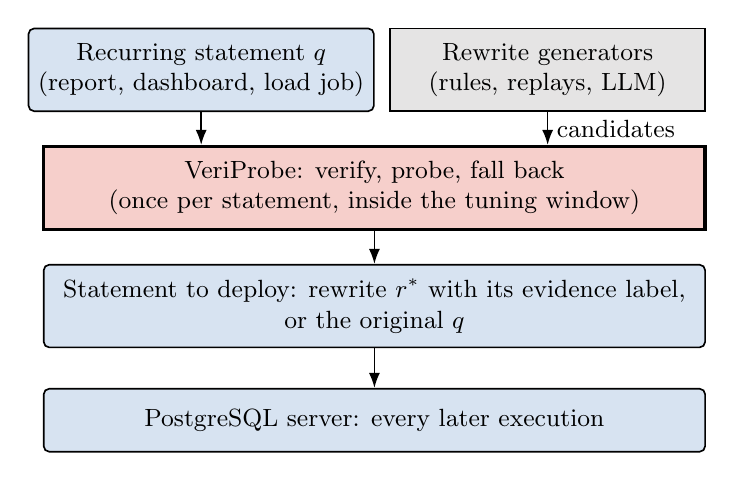
\begin{tikzpicture}[x=1cm,y=1cm]
  \node[store, minimum width=4.0cm, minimum height=1.05cm] (q) at (2.05, 4.55) {Recurring statement $q$\\(report, dashboard, load job)};
  \node[proc, minimum width=4.0cm, minimum height=1.05cm] (gen) at (6.45, 4.55) {Rewrite generators\\(rules, replays, LLM)};
  \node[exec, minimum width=8.4cm, minimum height=1.05cm] (sys) at (4.25, 3.05) {\sys{}: verify, probe, fall back\\(once per statement, inside the tuning window)};
  \node[store, minimum width=8.4cm, minimum height=1.05cm] (out) at (4.25, 1.55) {Statement to deploy: rewrite $r^{\ast}$ with its evidence label,\\or the original $q$};
  \node[store, minimum width=8.4cm, minimum height=0.8cm] (db) at (4.25, 0.10) {PostgreSQL server: every later execution};
  \draw[flow] (q.south) -- (q.south |- sys.north);
  \draw[flow] (gen.south) -- node[right, inner sep=3pt] {candidates} (gen.south |- sys.north);
  \draw[flow] (sys.south) -- (out.north);
  \draw[flow] (out.south) -- (db.north);
\end{tikzpicture}

  \caption{Application scenario. The layer runs once per recurring statement; the statement that it returns serves every later execution.}
  \label{fig:scenario}
\end{figure}

\textbf{Gap.}
Rewriters outside the DBMS do not meet these two conditions by themselves.
First, an LLM can produce a statement that is not equivalent, and a rule sequence replayed on a different schema can fail in the same way.
Second, a rewriter usually ranks its candidates by the planner's cost estimate, and estimates are unreliable for complex statements~\cite{leis2015}.
Recent tools add verification and execution feedback to a single generator: a tuning tool for Microsoft SQL Server verifies LLM rewrites with the optimizer and spends a time budget on execution~\cite{lee2026}, and ReSequel verifies LLM rewrites on sampled data and ranks them by performance~\cite{fathollahzadeh2026}.
Two questions remain open.
(i) Each system selects within its own candidate space, so it is unknown what a DBA gains from one verified selection step placed on top of several existing rewriters at once.
(ii) Rewriters are compared under time limits, and a run that exceeds its limit is commonly charged a fixed penalty. When the limit differs between the compared arms, the penalty decides the comparison, not the measurement.
Our logs show this effect directly: for one replayed arm, the charged value alone moves the result from a reduction of mean latency by \pc{\TpchHeldQuiteRedL} to an increase by \pc{\TpchHeldQuiteIncU}.

\textbf{Approach.}
We present \sys{}, a selection layer between rewrite generators and the DBMS.
\sys{} does not generate rewrites.
It takes a pool of candidates from any source, admits only candidates that pass an equivalence gate against the original statement, orders the admitted candidates by planner estimates without executing them, probes at most two of them with one bounded execution each, times the best probe fully, and returns the original statement unless that candidate is faster (Fig.~\ref{fig:overview}).
Every returned rewrite carries a label that states whether its equivalence evidence is a proof or bounded testing.
We evaluate \sys{} on the Transaction Processing Performance Council benchmark H (TPC-H), the decision support benchmark DSB, and the Calcite test workload.

\textbf{Findings.}
The evaluation supports three statements and contradicts the expectation that the layer outperforms each of its generators.
\begin{itemize}
\item On a development cohort of \DevN{} expensive statements, \sys{} improves \DevOursFaster{} statements and lowers mean latency from \secs{\DevOrigMean} to \secs{\DevOursMean}. The candidate pool of this cohort is tuned on the cohort, and its timings are assembled from several campaigns, so we treat it as an upper reference.
\item On \HeldAllN{} held-out statements, timed live, \sys{} improves \HeldAllOursFaster{} statements (\pc{\HeldAllOursFasterPct}) and lowers mean latency by \pc{\HeldAllOursRedU}. A validation session with one cutoff finds \ValHeldAllOursFaster{} of \ValHeldAllOursRewrites{} returned rewrites faster than the original.
\item \sys{} is robustly faster than a replay of the published QUITE rewrites on held-out statements, and robustly faster than both replays on skewed data.
\item \sys{} does not outperform a replay of the published R-Bot rewrites on held-out statements. In the validation session the mean latency of the replay is \secs{\ValHeldAllRbotMean} on the \ValHeldAllDone{} held-out pairs for which an arm returns a rewrite, against \secs{\ValHeldAllOursMean} for \sys{}. \sys{} keeps \ValHeldAllMissedOrigCutOff{} originals that are cut off although a replayed rewrite in its pool finishes; in turn it returns \ValHeldAllOursOnly{} faster rewrites where neither replay does.
\end{itemize}

\textbf{Contributions.}
\begin{itemize}
\item A selection layer for the scenario above that separates generation from admission and selection. Its inputs are heterogeneous: rule rewrites, replayed outputs of other systems, LLM proposals, and planner hints (Sections~\ref{sec:overview} and~\ref{sec:sources}).
\item An equivalence gate that fails closed and labels its evidence as syntactic, formal, or bounded (Section~\ref{sec:gate}).
\item A budgeted selection procedure with an explicit bound on the executions it adds on the target database, and a fallback that is anchored on the original statement (Section~\ref{sec:selection}).
\item An interval protocol for reporting rewrite latency under unequal cutoffs, with paired outcome classes that separate measured differences from undetermined ones, and a validation session that resolves them with one cutoff (Sections~\ref{sec:method} and~\ref{sec:rq7}).
\item An evaluation on \AllPairs{} pairs of database and statement that reports where the layer helps, where it does not, and which of its results hold only by construction (Sections~\ref{sec:results} and~\ref{sec:limits}).
\end{itemize}
The paper does not propose a new rewrite generator, and the layer combines known ingredients. Its novelty is the scenario specific combination and the measurement of what this combination adds to existing rewriters.

\begin{figure*}[t]
  \centering
  % Fig. 2: end-to-end data flow. Nodes are placed relative to each other with
% fixed gaps, so that no two nodes can overlap when the text changes.
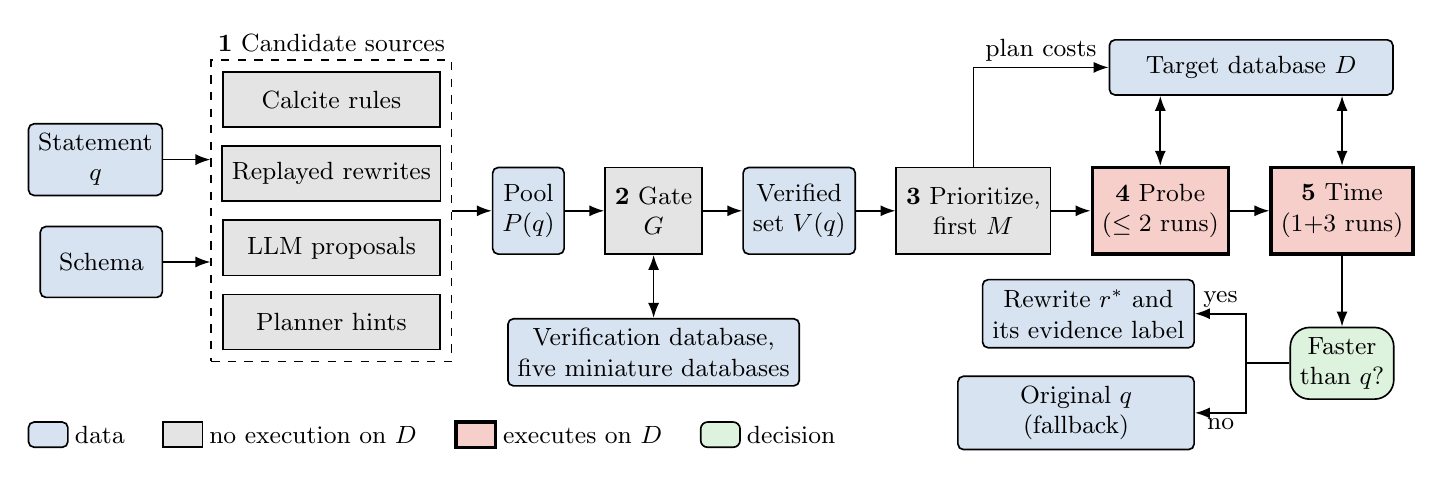
\begin{tikzpicture}[node distance=5mm]
  % step 1: candidate sources
  \node[proc, minimum width=2.75cm] (s1) {Calcite rules};
  \node[proc, minimum width=2.75cm, below=2.2mm of s1] (s2) {Replayed rewrites};
  \node[proc, minimum width=2.75cm, below=2.2mm of s2] (s3) {LLM proposals};
  \node[proc, minimum width=2.75cm, below=2.2mm of s3] (s4) {Planner hints};
  \begin{scope}[on background layer]
    \node[draw, line width=0.6pt, dashed, inner sep=4pt, fit=(s1)(s4)] (grp) {};
  \end{scope}
  \node[anchor=south, inner sep=2.5pt] at (grp.north) {\textbf{1}~Candidate sources};

  % inputs
  \node[store, minimum width=1.55cm, left=6mm of grp, yshift=6.5mm] (q) {Statement\\$q$};
  \node[store, minimum width=1.55cm, minimum height=9mm, left=6mm of grp, yshift=-6.5mm] (schema) {Schema};

  % main row
  \node[store, minimum height=11mm, right=of grp] (pool) {Pool\\$P(q)$};
  \node[proc, minimum height=11mm, right=of pool] (gate) {\textbf{2}~Gate\\$G$};
  \node[store, minimum height=11mm, right=of gate] (ver) {Verified\\set $V(q)$};
  \node[proc, minimum height=11mm, right=of ver] (prio) {\textbf{3}~Prioritize,\\first $M$};
  \node[exec, minimum height=11mm, right=of prio] (probe) {\textbf{4}~Probe\\($\le 2$ runs)};
  \node[exec, minimum height=11mm, right=of probe] (time) {\textbf{5}~Time\\($1{+}3$ runs)};

  % side stores
  \node[store, below=8mm of gate] (vdb) {Verification database,\\five miniature databases};
  \node[store, minimum width=3.6cm] (db) at ($(probe.north)!0.5!(time.north) + (0,1.25)$) {Target database $D$};

  % decision and outputs
  \node[dec, below=9mm of time] (dec) {Faster\\than $q$?};
  \node[store, left=12mm of dec, yshift=6.3mm] (out1) {Rewrite $r^{\ast}$ and\\its evidence label};
  \node[store, minimum width=3.0cm, left=12mm of dec, yshift=-6.3mm] (out2) {Original $q$\\(fallback)};

  % flows
  \draw[flow] (q.east) -- (q.east -| grp.west);
  \draw[flow] (schema.east) -- (schema.east -| grp.west);
  \draw[flow] (grp.east) -- (pool.west);
  \draw[flow] (pool.east) -- (gate.west);
  \draw[flow] (gate.east) -- (ver.west);
  \draw[flow] (ver.east) -- (prio.west);
  \draw[flow] (prio.east) -- (probe.west);
  \draw[flow] (probe.east) -- (time.west);
  \draw[biflow] (gate.south) -- (vdb.north);
  \draw[biflow] (probe.north) -- (probe.north |- db.south);
  \draw[biflow] (time.north) -- (time.north |- db.south);
  \draw[flow] (prio.north) |- node[pos=0.75, above, inner sep=2pt] {plan costs} (db.west);
  \draw[flow] (time.south) -- (dec.north);
  \draw[flow] (dec.west) -- ++(-0.55,0) |- node[pos=0.75, above, inner sep=2pt] {yes} (out1.east);
  \draw[flow] (dec.west) -- ++(-0.55,0) |- node[pos=0.75, below, inner sep=2pt] {no} (out2.east);

  % legend
  \coordinate (leg) at ([yshift=2mm]q.west |- out2.south);
  \node[store, minimum width=0.5cm, minimum height=0.32cm, inner sep=0pt, anchor=west] (l1) at (leg) {};
  \node[anchor=west, inner sep=2pt] (t1) at (l1.east) {data};
  \node[proc, minimum width=0.5cm, minimum height=0.32cm, inner sep=0pt, anchor=west] (l2) at ([xshift=4mm]t1.east) {};
  \node[anchor=west, inner sep=2pt] (t2) at (l2.east) {no execution on $D$};
  \node[exec, minimum width=0.5cm, minimum height=0.32cm, inner sep=0pt, anchor=west] (l3) at ([xshift=4mm]t2.east) {};
  \node[anchor=west, inner sep=2pt] (t3) at (l3.east) {executes on $D$};
  \node[dec, rounded corners=2.5pt, minimum width=0.5cm, minimum height=0.32cm, inner sep=0pt, anchor=west] (l4) at ([xshift=4mm]t3.east) {};
  \node[anchor=west, inner sep=2pt] (t4) at (l4.east) {decision};
\end{tikzpicture}

  \caption{Data flow of \sys{} for one statement. Steps 1 to 3 never execute a candidate on the target database; steps 4 and 5 execute at most two probes and one full timing.}
  \label{fig:overview}
\end{figure*}

% ===========================================================================
\section{Preliminaries and Problem Statement}
\label{sec:prelim}

\textbf{Statements and equivalence.}
A statement $q$ is a single read query over a schema $\Sigma$.
For a database instance $D$ of $\Sigma$, $q(D)$ denotes the result: a bag of rows, or a sequence of rows when $q$ has an outermost ordering.
Two statements $q$ and $p$ are equivalent, written $q \equiv p$, when $q(D') = p(D')$ for every instance $D'$ of $\Sigma$.
Deciding equivalence is undecidable for full SQL, so practical tools either prove it for a fragment~\cite{chu2017,zhou2019,zhou2022,ding2023,wang2024} or check it on a bounded set of instances~\cite{he2024}.

\textbf{Evidence classes.}
We distinguish three classes of evidence for $q \equiv p$: \emph{syntactic} (the two statements have the same tokens up to formatting and planner hints), \emph{formal} (a prover establishes equivalence for all instances), and \emph{bounded} (the results agree on a fixed finite set of instances, which can miss a difference that only other instances expose).

\textbf{Latency.}
The latency $\ell_{D}(q)$ is the execution time that the server reports for $q$ on $D$.
We measure it as the median of three runs after one warmup run.
Every run has a cutoff; a run that reaches its cutoff yields only a lower bound on the latency.

\textbf{Problem.}
Given a statement $q$, a target database $D$, and a pool $P(q)$ of candidate rewrites from arbitrary generators, the ideal output is
\begin{equation}
\left\{
\begin{aligned}
V(q) &= \{\, p \in P(q) : G(q,p) = 1 \,\},\\
r^{\ast} &= \operatorname*{arg\,min}_{r \in \{q\} \cup V(q)} \ell_{D}(r),
\end{aligned}
\right.
\label{eq:problem}
\end{equation}
where $q$ is the original statement, $P(q)$ is the candidate pool, $G(q,p) \in \{0,1\}$ is the decision of the equivalence gate for the pair $(q,p)$, $V(q)$ is the set of admitted candidates, $r^{\ast}$ is the statement to return, $D$ is the target database, and $\ell_{D}(r)$ is the latency of a statement $r$ on $D$.
The set $\{q\} \cup V(q)$ always contains $q$, so the output is never slower than the original when latencies are known exactly.
Latencies are known only through execution, and each execution on $D$ costs time inside the tuning window.
The problem is therefore to approximate~\eqref{eq:problem} with a bounded number of executions on $D$.

% ===========================================================================
\section{System Overview}
\label{sec:overview}

Fig.~\ref{fig:overview} shows the five steps of \sys{} and the data that flows between them.

Generators produce the pool $P(q)$ from the statement and the schema (step 1, Section~\ref{sec:sources}).
The gate checks each candidate against the original statement on a small verification database and on five miniature databases, and it labels each admitted candidate with its evidence (step 2, Section~\ref{sec:gate}).
\sys{} then orders the admitted candidates by planner estimates and keeps the first $M$ (step 3), probes at most two of them once on the target database (step 4), and times the fastest probe with the same protocol as the original, returning it only when it is faster (step 5, Section~\ref{sec:selection}).

\textbf{Running example.}
Fig.~\ref{fig:example} follows query 81 of DSB at scale factor 10, whose original run does not finish within \SI{\Tmax}{\second}.
The statement compares the total returns of every customer with 1.2 times the average total of the customer's state; the average is a correlated subquery.
The gate admits all \ExamplePool{} candidates of the pool.
An LLM proposal computes the averages per state once in a materialized common table expression (planner cost \ExampleMacroCost{}); the replayed R-Bot rewrite has planner cost \ExampleRuleCost{}.
Only the probe of the LLM proposal finishes; its full timing gives \SI{\ExampleOurs}{\second}, and \sys{} returns it with the label \emph{bounded}.

\begin{figure}[t]
  \centering
  % Fig. 3: the data that flows through the layer for one statement
% (DSB query 81, scale factor 10). Numbers come from the campaign log.
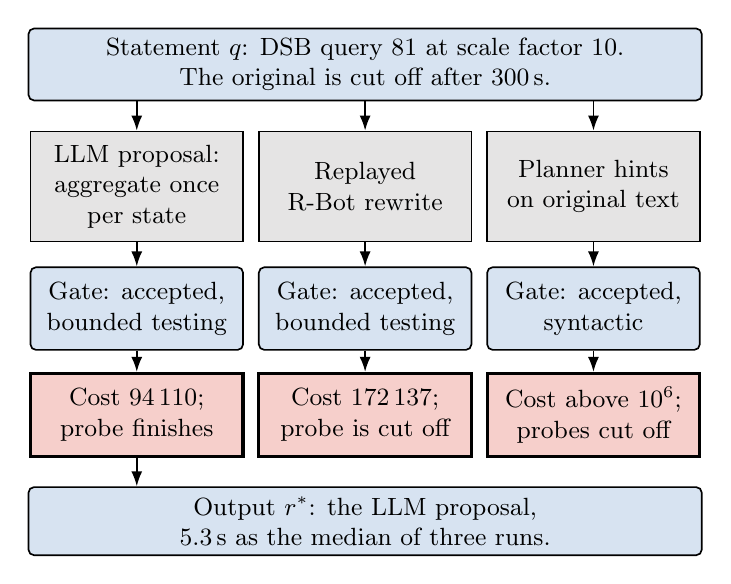
\begin{tikzpicture}[x=1cm,y=1cm]
  \node[store, minimum width=8.55cm] (q) at (4.275, 5.55)
    {Statement $q$: DSB query 81 at scale factor 10.\\The original is cut off after \SI{\Tmax}{\second}.};

  \node[proc, minimum width=2.70cm, minimum height=1.40cm] (c1) at (1.375, 4.00) {LLM proposal:\\aggregate once\\per state};
  \node[proc, minimum width=2.70cm, minimum height=1.40cm] (c2) at (4.275, 4.00) {Replayed\\R-Bot rewrite};
  \node[proc, minimum width=2.70cm, minimum height=1.40cm] (c3) at (7.175, 4.00) {Planner hints\\on original text};

  \node[store, minimum width=2.70cm, minimum height=1.05cm] (g1) at (1.375, 2.45) {Gate: accepted,\\bounded testing};
  \node[store, minimum width=2.70cm, minimum height=1.05cm] (g2) at (4.275, 2.45) {Gate: accepted,\\bounded testing};
  \node[store, minimum width=2.70cm, minimum height=1.05cm] (g3) at (7.175, 2.45) {Gate: accepted,\\syntactic};

  \node[exec, minimum width=2.70cm, minimum height=1.05cm] (p1) at (1.375, 1.10) {Cost \ExampleMacroCost;\\probe finishes};
  \node[exec, minimum width=2.70cm, minimum height=1.05cm] (p2) at (4.275, 1.10) {Cost \ExampleRuleCost;\\probe is cut off};
  \node[exec, minimum width=2.70cm, minimum height=1.05cm] (p3) at (7.175, 1.10) {Cost above $10^{6}$;\\probes cut off};

  \node[store, minimum width=8.55cm] (r) at (4.275, -0.25)
    {Output $r^{\ast}$: the LLM proposal,\\\SI{\ExampleOurs}{\second} as the median of three runs.};

  \foreach \c in {c1,c2,c3} {\draw[flow] (\c.north |- q.south) -- (\c.north);}
  \draw[flow] (c1.south) -- (g1.north);
  \draw[flow] (c2.south) -- (g2.north);
  \draw[flow] (c3.south) -- (g3.north);
  \draw[flow] (g1.south) -- (p1.north);
  \draw[flow] (g2.south) -- (p2.north);
  \draw[flow] (g3.south) -- (p3.north);
  \draw[flow] (p1.south) -- (p1.south |- r.north);
\end{tikzpicture}

  \caption{Data flow for DSB query 81 at scale factor 10. Four admitted candidates that combine a rewrite with a planner hint are omitted; their probes are cut off or fail.}
  \label{fig:example}
\end{figure}

% ===========================================================================
\section{Candidate Sources}
\label{sec:sources}

\sys{} distinguishes two classes of candidates by how they are produced.

\textbf{Class A: rule rewrites.}
A class A candidate is the output of Apache Calcite rules~\cite{begoli2018} applied to the original statement.
We obtain these candidates in three ways: (i) the rewritten statements of R-Bot that ship with the public QUITE repository, (ii) rule sequences from the released R-Bot logs, which we apply again through the Calcite executor that R-Bot ships, and (iii) single Calcite rules whose pattern matches the statement, used only when (i) and (ii) yield nothing and only in campaigns that include Calcite statements.

\textbf{Class B: free rewrites and planner hints.}
A class B candidate is a statement that no fixed rule set produces.
We use three kinds.
(i) \emph{LLM proposals.} A language model receives the statement, the schema, and a plan from a small development database, and proposes rewritten statements. We generate all proposals once, before any timing on the target databases, and freeze them in a file: 666 proposals for 439 distinct statements. The generation inspects neither published rewrites nor latencies on the target databases.
(ii) \emph{Replayed QUITE rewrites.} We take the rewritten statements that the QUITE authors publish~\cite{song2025}.
(iii) \emph{Planner hints.} A candidate keeps the text of a statement and adds a comment that the pg\_hint\_plan extension~\cite{pghintplan} interprets, for example to disable nested loop joins for this statement. A hint changes the plan and never the result; steering the optimizer with hints is an established technique~\cite{marcus2021}.

\textbf{Composition.}
A candidate that is produced from another candidate has depth 2 or more.
The gate always compares a candidate with the original statement, never with its parent, so an error cannot accumulate along a chain.

\textbf{Pool construction.}
Fig.~\ref{fig:pool} shows how the pool of one statement is built.
The runner first collects the frozen LLM proposals and the published rewrites that are stored for the text of $q$.
If no rule rewrite is among them, it applies up to eight matching Calcite rules, one rule at a time.
The runner also normalizes count aggregates over columns that are declared not null, which adds one more candidate where it applies.
The runner then treats every new candidate like $q$: it looks up proposals for the text of the candidate, and for the \SeededQueries{} statements of the development cohort that Section~\ref{sec:setup} describes it adds planner hints.
Expansion stops when no new candidate appears or when depth five is reached.
Finally the runner removes duplicate texts and keeps at most 64 candidates.
In our campaigns the largest pool holds \MaxPool{} candidates, no admitted candidate is deeper than \MaxDepth{}, and \EmptyPools{} statements, all of them TPC-H statements, have an empty pool.

\begin{figure}[t]
  \centering
  % Flowchart: how the candidate pool of one statement is built.
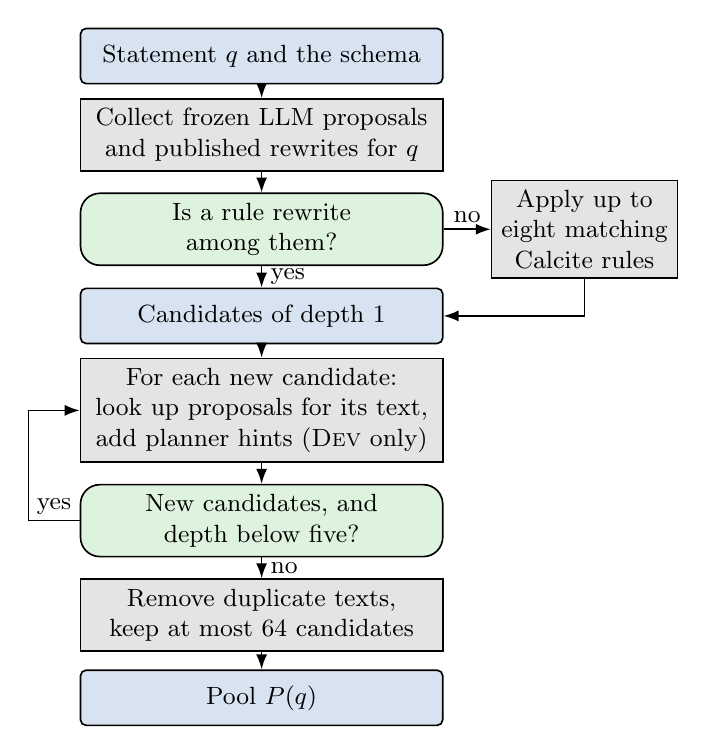
\begin{tikzpicture}[x=1cm,y=1cm]
  \node[store, minimum width=4.6cm] (in) at (0, 7.85) {Statement $q$ and the schema};
  \node[proc, minimum width=4.6cm] (collect) at (0, 6.85) {Collect frozen LLM proposals\\and published rewrites for $q$};
  \node[dec, minimum width=4.6cm] (rule) at (0, 5.65) {Is a rule rewrite\\among them?};
  \node[proc, minimum width=2.3cm] (calcite) at (4.10, 5.65) {Apply up to\\eight matching\\Calcite rules};
  \node[store, minimum width=4.6cm] (d1) at (0, 4.55) {Candidates of depth 1};
  \node[proc, minimum width=4.6cm] (expand) at (0, 3.35) {For each new candidate:\\look up proposals for its text,\\add planner hints (\textsc{Dev} only)};
  \node[dec, minimum width=4.6cm] (more) at (0, 1.95) {New candidates, and\\depth below five?};
  \node[proc, minimum width=4.6cm] (dedup) at (0, 0.75) {Remove duplicate texts,\\keep at most 64 candidates};
  \node[store, minimum width=4.6cm] (pool) at (0, -0.30) {Pool $P(q)$};

  \draw[flow] (in.south) -- (collect.north);
  \draw[flow] (collect.south) -- (rule.north);
  \draw[flow] (rule.south) -- node[right, inner sep=3pt] {yes} (d1.north);
  \draw[flow] (rule.east) -- node[above, inner sep=2pt] {no} (calcite.west);
  \draw[flow] (calcite.south) |- (d1.east);
  \draw[flow] (d1.south) -- (expand.north);
  \draw[flow] (expand.south) -- (more.north);
  \draw[flow] (more.west) -- node[above, inner sep=2pt] {yes} ++(-0.65,0) |- (expand.west);
  \draw[flow] (more.south) -- node[right, inner sep=3pt] {no} (dedup.north);
  \draw[flow] (dedup.south) -- (pool.north);
\end{tikzpicture}

  \caption{Construction of the candidate pool $P(q)$ for one statement. Planner hints are added only for statements of the development cohort.}
  \label{fig:pool}
\end{figure}

% ===========================================================================
\section{Equivalence Gate}
\label{sec:gate}

The gate decides $G(q,p)$ for a pair of statements and returns an evidence label.
It fails closed: an unsupported construct, an error, or an inconclusive result rejects the candidate.
Fig.~\ref{fig:gate} shows the decision flow.

\begin{figure}[t]
  \centering
  % Fig. 5: decision flow of the equivalence gate.
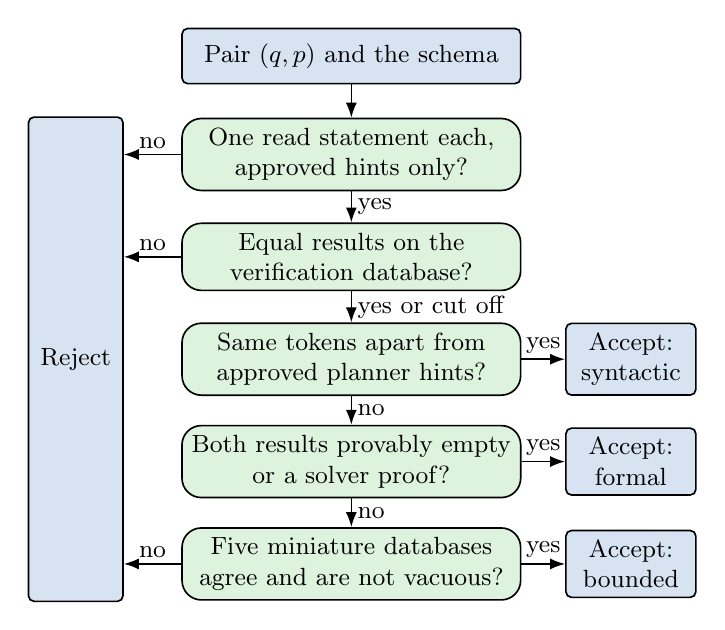
\begin{tikzpicture}[x=1cm,y=1cm]
  \node[store, minimum width=4.3cm] (in) at (0, 6.60) {Pair $(q, p)$ and the schema};
  \node[dec, minimum width=4.3cm] (d0) at (0, 5.35) {One read statement each,\\approved hints only?};
  \node[dec, minimum width=4.3cm] (d1) at (0, 4.05) {Equal results on the\\verification database?};
  \node[dec, minimum width=4.3cm] (d2) at (0, 2.75) {Same tokens apart from\\approved planner hints?};
  \node[dec, minimum width=4.3cm] (d3) at (0, 1.45) {Both results provably empty\\or a solver proof?};
  \node[dec, minimum width=4.3cm] (d4) at (0, 0.15) {Five miniature databases\\agree and are not vacuous?};

  \node[store, minimum width=1.65cm] (a2) at (3.55, 2.75) {Accept:\\syntactic};
  \node[store, minimum width=1.65cm] (a3) at (3.55, 1.45) {Accept:\\formal};
  \node[store, minimum width=1.65cm] (a4) at (3.55, 0.15) {Accept:\\bounded};
  \node[store, minimum width=1.2cm, minimum height=6.15cm] (rej) at (-3.50, 2.75) {Reject};

  \draw[flow] (in.south) -- (d0.north);
  \draw[flow] (d0.south) -- node[right, inner sep=2pt] {yes} (d1.north);
  \draw[flow] (d1.south) -- node[right, inner sep=2pt] {yes or cut off} (d2.north);
  \draw[flow] (d2.south) -- node[right, inner sep=2pt] {no} (d3.north);
  \draw[flow] (d3.south) -- node[right, inner sep=2pt] {no} (d4.north);
  \draw[flow] (d2.east) -- node[above, inner sep=2pt] {yes} (a2.west);
  \draw[flow] (d3.east) -- node[above, inner sep=2pt] {yes} (a3.west);
  \draw[flow] (d4.east) -- node[above, inner sep=2pt] {yes} (a4.west);
  \draw[flow] (d0.west) -- node[above, inner sep=2pt] {no} (d0.west -| rej.east);
  \draw[flow] (d1.west) -- node[above, inner sep=2pt] {no} (d1.west -| rej.east);
  \draw[flow] (d4.west) -- node[above, inner sep=2pt] {no} (d4.west -| rej.east);
\end{tikzpicture}

  \caption{Decision flow of the equivalence gate. A candidate is admitted only through one of the three accepting exits, and the exit determines its evidence label.}
  \label{fig:gate}
\end{figure}

\textbf{Admissible input.}
Each side must parse as exactly one read statement.
A planner hint is admissible only when it belongs to an approved list of plan directives: join methods, scan methods, join order, and planner switches.
A comment that can change results is rejected.

\textbf{Execution check.}
The gate executes both statements on a verification database in one snapshot and compares the results as bags, or as sequences when the statement orders its output.
The verification database has the schema of the target database and little data: TPC-H at scale factor 0.01, DSB at scale factor 1, and \num{10000} rows per main table for the Calcite schema.
The gate first confirms that both databases have the same tables, columns, types, keys, and collations.
The comparison is positional and tolerates a relative numeric difference of $10^{-5}$.
Unequal results reject the candidate.
If the comparison exceeds its time limit, the gate continues with the remaining checks, because a slow original is not evidence against equivalence.

\textbf{Syntactic exit.}
If the two statements have the same token sequence apart from approved planner hints, the gate accepts with the label \emph{syntactic}.

\textbf{Formal exit.}
Two provers can accept.
The first is SQLSolver~\cite{ding2023}, which the gate calls only for a restricted fragment: select, project, join, set operations, and Boolean predicates over integer and text columns, with all key and null constraints removed from the schema that the prover receives.
The second is a structural check for one pattern: both statements provably return no row, for example because a filter requires a window count to be null.
A prover verdict of not equivalent rejects the candidate.

\textbf{Bounded exit.}
Otherwise the gate runs both statements on five miniature databases that it builds from the schema and from the literals of the statement: an empty database, one with null values, one with duplicate rows, one with skewed values, and one with unmatched join keys.
The gate accepts with the label \emph{bounded} when all five results agree and the evidence is not vacuous: at least one miniature must return rows, and the five results must not all be identical.

\textbf{What the gate does not establish.}
The labels \emph{syntactic} and \emph{formal} cover all instances.
The label \emph{bounded} covers six instances.
The gate never compares results on the target database; Section~\ref{sec:rq6} reports how often each label occurs.

% ===========================================================================
\section{Budgeted Selection with Fallback}
\label{sec:selection}

The selection procedure approximates~\eqref{eq:problem} with few executions on the target database.

\textbf{Prioritization.}
Each admitted candidate $p \in V(q)$ receives the key
\begin{equation}
\pi(p) = \bigl(d(p),\; \mathbf{1}[\kappa(p) \ge \kappa(q)],\; b(p),\; \kappa(p),\; i(p)\bigr),
\label{eq:priority}
\end{equation}
where $\pi(p)$ is the key, $d(p)$ is the depth of $p$, $\kappa(\cdot)$ is the total cost that the planner of the target database estimates for a statement, $\mathbf{1}[\cdot]$ equals 1 when its argument holds and 0 otherwise, $b(p)$ equals 0 when the action that produces $p$ or the estimated plan of $p$ involves a join, a nested loop, a subplan, a materialization, or a decorrelation, and 1 otherwise, and $i(p)$ is the position of $p$ in the order of generation.
\sys{} sorts $V(q)$ by $\pi$ in ascending lexicographic order and keeps the first $M$ candidates as the prefix $V_{M}(q)$.
The order uses only planner estimates and is fixed before any candidate executes.

\textbf{Probes.}
A probe is one execution of a candidate on the target database, without a warmup run, with the cutoff
\begin{equation}
c_{\mathrm{p}}(q) = \min\bigl(\ell_{0}(q),\, \bar{c}\bigr),
\label{eq:probe}
\end{equation}
where $c_{\mathrm{p}}(q)$ is the probe cutoff, $\ell_{0}(q)$ is the measured latency of the original statement, set to the timeout $T_{\max}$ when the original is cut off, and $\bar{c}$ is a fixed cap.
We use $T_{\max} = \SI{\Tmax}{\second}$ and $\bar{c} = \SI{45}{\second}$; for five statements of the development cohort with long originals, $\bar{c} = \SI{120}{\second}$.
\sys{} walks through $V_{M}(q)$ in priority order and probes at most two candidates.
It reuses a result without a new execution in two cases: a timing of the same statement text exists in the measurement cache, or the candidate has the same estimated plan as a statement that is already timed.
After one probe improves on the original by more than \SI{15}{\percent}, \sys{} skips candidates that carry no planner hint and whose planner cost is not below that of the original.

\textbf{Timing and decision.}
Let $\tilde{\ell}(p)$ denote the probe time of $p$ and $\ell(p)$ the median of three timed runs of $p$ under the cutoff
\begin{equation}
c_{\mathrm{f}}(q) = \min\bigl(T_{\max},\, \max(\SI{60}{\second},\, 1.05\,\ell_{0}(q))\bigr),
\label{eq:final}
\end{equation}
where $c_{\mathrm{f}}(q)$ is the cutoff of the timed runs, and $T_{\max}$ and $\ell_{0}(q)$ are as in~\eqref{eq:probe}.
The output of \sys{} is
\begin{equation}
\left\{
\begin{aligned}
S(q) &= \{\, p \in V_{M}(q) : \tilde{\ell}(p) < \ell_{0}(q) \,\},\\
p^{\ast} &= \operatorname*{arg\,min}_{p \in S(q)} \tilde{\ell}(p),\\
r^{\ast} &=
  \begin{cases}
    p^{\ast}, & S(q) \neq \emptyset \text{ and } \ell(p^{\ast}) < \ell_{0}(q),\\
    q, & \text{otherwise},
  \end{cases}
\end{aligned}
\right.
\label{eq:decision}
\end{equation}
where $S(q)$ is the set of probed candidates that finish faster than the original, $p^{\ast}$ is the fastest probe, and $r^{\ast}$ is the returned statement.
When a second member of $S(q)$ already has a full timing in the cache, \sys{} compares both full timings and keeps the faster one.
A probe that takes at least \SI{10}{\second} counts as the first of the three timed runs, so that a long candidate executes three times in total.
Fig.~\ref{fig:selection} shows the control flow of the procedure, and Fig.~\ref{fig:timeline} shows the executions that it places on the target database.
In Fig.~\ref{fig:selection} the two steps with a heavy outline are the only ones that execute a candidate on $D$.

\begin{figure*}[t]
  \centering
  % Flowchart of the selection procedure (Algorithm 1), two rows.
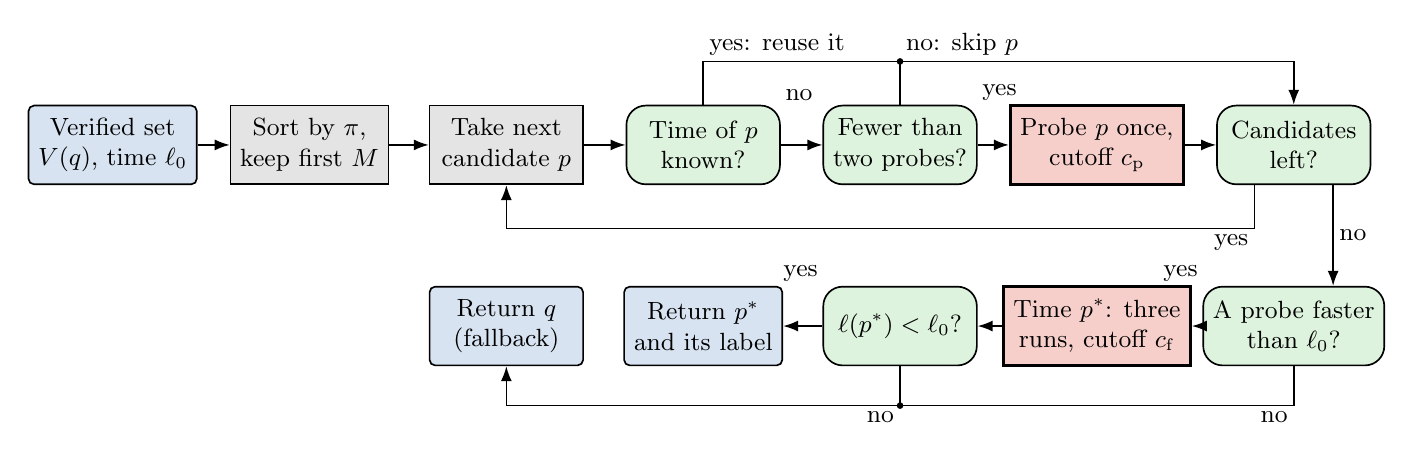
\begin{tikzpicture}[x=1cm,y=1cm]
  \foreach \i/\x in {1/1.05, 2/3.55, 3/6.05, 4/8.55, 5/11.05, 6/13.55, 7/16.05} {\coordinate (c\i) at (\x, 0);}
  % row 1
  \node[store, minimum width=1.95cm, minimum height=1.0cm] (n1) at (1.05, 2.3) {Verified set\\$V(q)$, time $\ell_{0}$};
  \node[proc, minimum width=1.95cm, minimum height=1.0cm] (n2) at (3.55, 2.3) {Sort by $\pi$,\\keep first $M$};
  \node[proc, minimum width=1.95cm, minimum height=1.0cm] (n3) at (6.05, 2.3) {Take next\\candidate $p$};
  \node[dec, minimum width=1.95cm, minimum height=1.0cm] (n4) at (8.55, 2.3) {Time of $p$\\known?};
  \node[dec, minimum width=1.95cm, minimum height=1.0cm] (n5) at (11.05, 2.3) {Fewer than\\two probes?};
  \node[exec, minimum width=1.95cm, minimum height=1.0cm] (n6) at (13.55, 2.3) {Probe $p$ once,\\cutoff $c_{\mathrm{p}}$};
  \node[dec, minimum width=1.95cm, minimum height=1.0cm] (n7) at (16.05, 2.3) {Candidates\\left?};
  % row 2
  \node[dec, minimum width=1.95cm, minimum height=1.0cm] (m7) at (16.05, 0) {A probe faster\\than $\ell_{0}$?};
  \node[exec, minimum width=1.95cm, minimum height=1.0cm] (m6) at (13.55, 0) {Time $p^{\ast}$: three\\runs, cutoff $c_{\mathrm{f}}$};
  \node[dec, minimum width=1.95cm, minimum height=1.0cm] (m5) at (11.05, 0) {$\ell(p^{\ast}) < \ell_{0}$?};
  \node[store, minimum width=1.95cm, minimum height=1.0cm] (m4) at (8.55, 0) {Return $p^{\ast}$\\and its label};
  \node[store, minimum width=1.95cm, minimum height=1.0cm] (m3) at (6.05, 0) {Return $q$\\(fallback)};

  \draw[flow] (n1.east) -- (n2.west);
  \draw[flow] (n2.east) -- (n3.west);
  \draw[flow] (n3.east) -- (n4.west);
  \draw[flow] (n4.east) -- (n5.west);
  \node[anchor=south west, inner sep=1.5pt] at (n4.north east) {no};
  \draw[flow] (n5.east) -- (n6.west);
  \node[anchor=south west, inner sep=1.5pt] at (n5.north east) {yes};
  \draw[flow] (n6.east) -- (n7.west);
  % known time or no probe left: go on without a probe
  \draw[flow] (n4.north) -- ++(0,0.55) -| (n7.north);
  \node[anchor=south west, inner sep=2pt] at ([yshift=0.55cm]n4.north) {yes: reuse it};
  \draw[line width=0.6pt] (n5.north) -- ++(0,0.55);
  \fill ([yshift=0.55cm]n5.north) circle (1.2pt);
  \node[anchor=south west, inner sep=2pt] at ([yshift=0.55cm]n5.north) {no: skip $p$};
  % loop
  \draw[flow] ([xshift=-5mm]n7.south) -- ++(0,-0.55) -| (n3.south);
  \node[anchor=north east, inner sep=2pt] at ([xshift=-5mm,yshift=-0.55cm]n7.south) {yes};
  \draw[flow] ([xshift=5mm]n7.south) -- node[right, inner sep=2pt] {no} ([xshift=5mm]m7.north);
  % row 2
  \draw[flow] (m7.west) -- (m6.east);
  \node[anchor=south east, inner sep=1.5pt] at (m7.north west) {yes};
  \draw[flow] (m6.west) -- (m5.east);
  \draw[flow] (m5.west) -- (m4.east);
  \node[anchor=south east, inner sep=1.5pt] at (m5.north west) {yes};
  \draw[flow] (m7.south) -- ++(0,-0.5) -| (m3.south);
  \node[anchor=north east, inner sep=2pt] at ([yshift=-0.5cm]m7.south) {no};
  \draw[line width=0.6pt] (m5.south) -- ++(0,-0.5);
  \fill ([yshift=-0.5cm]m5.south) circle (1.2pt);
  \node[anchor=north east, inner sep=2pt] at ([yshift=-0.5cm]m5.south) {no};
\end{tikzpicture}

  \caption{Control flow of the selection procedure with budget $M$. Node styles are those of Fig.~\ref{fig:overview}; steps with a heavy outline execute on the target database.}
  \label{fig:selection}
\end{figure*}

\begin{figure}[t]
  \centering
  % Fig. 7: what runs on the target database for one statement, in order.
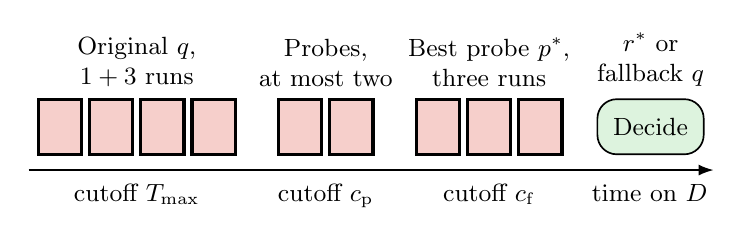
\begin{tikzpicture}[x=1cm,y=1cm]
  \draw[flow] (0.00, 0.00) -- (8.70, 0.00);
  \node[anchor=north east, inner sep=2pt] at (8.70, -0.10) {time on $D$};

  \foreach \i/\x in {0/0.40, 1/1.05, 2/1.70, 3/2.35} {
    \node[exec, minimum width=0.55cm, minimum height=0.70cm, inner sep=0pt] (o\i) at (\x, 0.55) {};}
  \node[anchor=south, inner sep=2pt, align=center] at (1.375, 0.98) {Original $q$,\\$1 + 3$ runs};

  \node[exec, minimum width=0.55cm, minimum height=0.70cm, inner sep=0pt] (p1) at (3.45, 0.55) {};
  \node[exec, minimum width=0.55cm, minimum height=0.70cm, inner sep=0pt] (p2) at (4.10, 0.55) {};
  \node[anchor=south, inner sep=2pt, align=center] at (3.775, 0.98) {Probes,\\at most two};

  \foreach \i/\x in {1/5.20, 2/5.85, 3/6.50} {
    \node[exec, minimum width=0.55cm, minimum height=0.70cm, inner sep=0pt] (f\i) at (\x, 0.55) {};}
  \node[anchor=south, inner sep=2pt, align=center] at (5.85, 0.98) {Best probe $p^{\ast}$,\\three runs};

  \node[dec, minimum width=1.35cm, minimum height=0.70cm] (d) at (7.90, 0.55) {Decide};
  \node[anchor=south, inner sep=2pt, align=center] at (7.90, 0.98) {$r^{\ast}$ or\\fallback $q$};

  \node[anchor=north, inner sep=2pt] at (1.375, -0.10) {cutoff $T_{\max}$};
  \node[anchor=north, inner sep=2pt] at (3.775, -0.10) {cutoff $c_{\mathrm{p}}$};
  \node[anchor=north, inner sep=2pt] at (5.85, -0.10) {cutoff $c_{\mathrm{f}}$};
\end{tikzpicture}

  \caption{Executions that \sys{} places on the target database $D$ for one statement. Each box is one run; the cutoffs are those of~\eqref{eq:probe} and~\eqref{eq:final}.}
  \label{fig:timeline}
\end{figure}

\textbf{Cost bound.}
Beyond the timing of the original statement, the executions that \sys{} adds on $D$ take at most
\begin{equation}
C(q) \le 2\,c_{\mathrm{p}}(q) + 4\,\ell(p^{\ast}),
\label{eq:cost}
\end{equation}
where $C(q)$ is the time of these executions, $c_{\mathrm{p}}(q)$ is the probe cutoff of~\eqref{eq:probe}, and $\ell(p^{\ast})$ is the latency of the fully timed candidate, counted four times for one warmup and three runs.
A rewrite that saves $\ell_{0}(q) - \ell(r^{\ast})$ per execution recovers this cost after
\begin{equation}
n(q) = \frac{C(q)}{\ell_{0}(q) - \ell(r^{\ast})}
\label{eq:amortize}
\end{equation}
executions, where $n(q)$ is this number of executions, $C(q)$ is the bound of~\eqref{eq:cost}, $\ell_{0}(q)$ is the latency of the original, and $\ell(r^{\ast})$ is the latency of the returned rewrite.

\textbf{Properties.}
Two properties follow from~\eqref{eq:decision} and do not depend on the quality of the candidates: the returned statement is the original or an admitted candidate, and it is not slower than the original in the three timed runs that \sys{} compares.
The second property holds for these runs; it is not a prediction for later executions (Section~\ref{sec:rq7}).

% ===========================================================================
\section{Evaluation Methodology}
\label{sec:method}

\subsection{Setup}
\label{sec:setup}

\textbf{Server.}
All experiments run on one workstation with an Intel Core i5-12450H processor (8 cores), \SI{31}{\gibi\byte} of main memory, and Ubuntu 24.04.
The DBMS is PostgreSQL 14.13 with the pg\_hint\_plan extension, \SI{256}{\mebi\byte} of shared buffers, \SI{8}{\mebi\byte} of working memory per operation, parallel query execution disabled, and just-in-time compilation disabled.
This configuration is small for the data sizes below, and it makes many original statements slow.
We keep it fixed for all arms.

\textbf{Data.}
We use TPC-H~\cite{tpch} at scale factors (SF) 10 and 50, DSB~\cite{ding2021} at SF 10 and 50, and the schema of the Calcite test suite filled with 40 million rows per main table by the generator of SlabCity~\cite{dong2023}, once with uniform and once with Zipf distributed values.

\textbf{Statements.}
The public repositories of R-Bot and QUITE contain 441 statements for these schemas: 107 for TPC-H, 232 for DSB, and 102 for Calcite.
We evaluate all 107 TPC-H statements, the 44 Calcite statements of R-Bot, and 10 DSB statements.
The remaining 222 DSB statements and the 58 Calcite statements of QUITE are not evaluated (Section~\ref{sec:limits}).

\textbf{Cohorts.}
Table~\ref{tab:cohorts} lists the five cohorts.
\textsc{Dev} contains 10 R-Bot statements each for TPC-H at SF 10, DSB at SF 10, and Calcite with uniform data. They are chosen before any timing by descending planner cost, one statement per query family, below a cost ceiling that excludes plans the planner rates as pathological.
The pool is developed on \textsc{Dev}: for \SeededQueries{} of its statements it contains planner hints that we add after inspecting their plans, for one statement it contains one rewrite that we write manually, and it contains 32 candidates collected in earlier runs on these statements.
The two held-out cohorts contain all other evaluated TPC-H and Calcite statements; the pool of a held-out statement contains no manually added candidate.
\textsc{Zipf} runs the first 30 Calcite statements on skewed data, and \textsc{SF\,50} runs the 20 TPC-H and DSB statements of \textsc{Dev} on five times more data.
Fig.~\ref{fig:workflow} shows the order of these steps.

\begin{figure}[t]
  \centering
  % Order of the experimental steps.
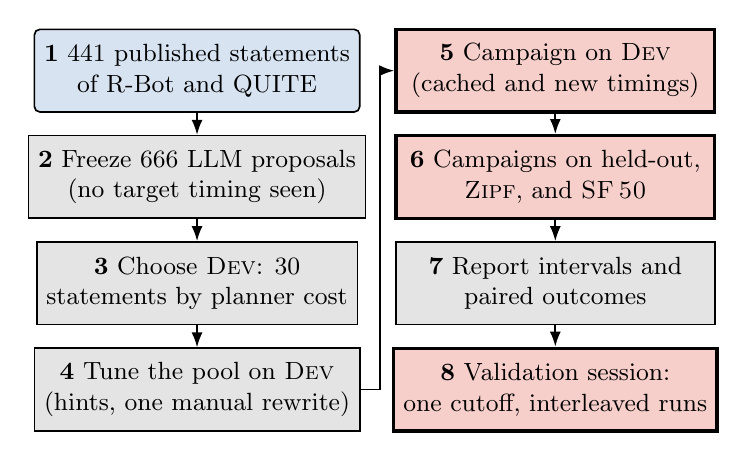
\begin{tikzpicture}[x=1cm,y=1cm]
  \node[store, minimum width=4.05cm, minimum height=1.05cm] (s1) at (2.05, 4.05) {\textbf{1}~441 published statements\\of R-Bot and QUITE};
  \node[proc, minimum width=4.05cm, minimum height=1.05cm] (s2) at (2.05, 2.70) {\textbf{2}~Freeze 666 LLM proposals\\(no target timing seen)};
  \node[proc, minimum width=4.05cm, minimum height=1.05cm] (s3) at (2.05, 1.35) {\textbf{3}~Choose \textsc{Dev}: 30\\statements by planner cost};
  \node[proc, minimum width=4.05cm, minimum height=1.05cm] (s4) at (2.05, 0.00) {\textbf{4}~Tune the pool on \textsc{Dev}\\(hints, one manual rewrite)};
  \node[exec, minimum width=4.05cm, minimum height=1.05cm] (s5) at (6.60, 4.05) {\textbf{5}~Campaign on \textsc{Dev}\\(cached and new timings)};
  \node[exec, minimum width=4.05cm, minimum height=1.05cm] (s6) at (6.60, 2.70) {\textbf{6}~Campaigns on held-out,\\\textsc{Zipf}, and \textsc{SF\,50}};
  \node[proc, minimum width=4.05cm, minimum height=1.05cm] (s7) at (6.60, 1.35) {\textbf{7}~Report intervals and\\paired outcomes};
  \node[exec, minimum width=4.05cm, minimum height=1.05cm] (s8) at (6.60, 0.00) {\textbf{8}~Validation session:\\one cutoff, interleaved runs};
  \draw[flow] (s1.south) -- (s2.north);
  \draw[flow] (s2.south) -- (s3.north);
  \draw[flow] (s3.south) -- (s4.north);
  \draw[flow] (s4.east) -- ++(0.25,0) |- (s5.west);
  \draw[flow] (s5.south) -- (s6.north);
  \draw[flow] (s6.south) -- (s7.north);
  \draw[flow] (s7.south) -- (s8.north);
\end{tikzpicture}

  \caption{Order of the experimental steps. Steps with a heavy outline execute statements on the target databases.}
  \label{fig:workflow}
\end{figure}

\begin{table}[t]
\caption{Cohorts. Size: number of statements. Live: number of original statements that are timed in the same campaign as their candidates.}
\label{tab:cohorts}
\centering
\footnotesize
\begin{tabular}{@{}llrr@{}}
\toprule
Cohort & Databases & Size & Live \\
\midrule
\textsc{Dev} & TPC-H, DSB, Calcite & \DevN & \DevOrigLive \\
\textsc{TPC-H} held-out & TPC-H, SF 10 & \TpchHeldN & \TpchHeldOrigLive \\
\textsc{Calcite} held-out & Calcite, uniform & \CalciteHeldN & \CalciteHeldOrigLive \\
\textsc{Zipf} & Calcite, Zipf & \ZipfN & \ZipfOrigLive \\
\textsc{SF\,50} & TPC-H and DSB, SF 50 & \SfFiftyN & \SfFiftyOrigLive \\
\bottomrule
\end{tabular}
\end{table}

\textbf{Arms.}
We compare four arms on every statement.
\emph{Original} is the unchanged statement.
\emph{\sys{}} is the procedure of Fig.~\ref{fig:selection} with $M = 16$ on the full pool.
\emph{R-Bot replay} returns the admitted rule rewrite of Section~\ref{sec:sources} with the lowest planner cost, provided that this cost is below the cost of the original; it selects without probes and has no fallback.
\emph{QUITE replay} returns the first admitted published QUITE rewrite, also without probes and without fallback.
Both replay arms return the original statement when they have no admitted candidate.
The replay arms are not runs of R-Bot and QUITE: their language model calls, retrieval, and feedback loops do not execute in our study.
They measure what the published rewrites of these systems achieve when a DBA applies them on a different server after our gate.

\textbf{Timing.}
Latency is the execution time that the PostgreSQL server reports when it executes a statement under its plan analysis command, with timing of individual plan nodes switched off.
The original statement runs with the cutoff $T_{\max}$; every other statement runs with the cutoff of~\eqref{eq:final}.
A replay arm does not time its rewrite directly. It first runs the rewrite once with a cutoff between \SI{60}{\second} and \SI{120}{\second}, or it reuses the probe of \sys{} when \sys{} has probed the same statement, and it times the rewrite fully only when this run finishes.
At SF 50, an original whose run at SF 10 is cut off runs with a cutoff of \SI{120}{\second}.
All LLM proposals come from one model, recorded in the artifact as gpt-6.1-sol.
A measurement cache keyed by database and statement text avoids timing the same text twice.
Code, manifests, frozen proposals, and raw logs are available at \url{https://github.com/terraspacer/VeriProbe}.

\subsection{Interval Reporting under Unequal Cutoffs}
\label{sec:intervals}

A run that is cut off after $c$ seconds shows only that the latency is at least $c$.
Reports on query rewriting usually replace such a run by $T_{\max}$.
This is harmless when every arm has the cutoff $T_{\max}$.
It is not harmless in our logs, where the cutoff of a run ranges from the probe cutoff of~\eqref{eq:probe} to \SI{\Tmax}{\second}: a rewrite that is stopped after \SI{20}{\second} and charged \SI{\Tmax}{\second} is charged \PenaltyFactor{} times the time for which it is observed.
We therefore keep both ends of the interval.
For an arm $s$ and a statement $q$,
\begin{equation}
\bigl(\ell^{L}_{s}(q),\, \ell^{U}_{s}(q)\bigr) =
\begin{cases}
\bigl(m_{s}(q),\, m_{s}(q)\bigr), & \text{if the runs finish},\\
\bigl(c_{s}(q),\, T_{\max}\bigr), & \text{if the runs are cut off},
\end{cases}
\label{eq:interval}
\end{equation}
where $\ell^{L}_{s}(q)$ and $\ell^{U}_{s}(q)$ are the lower and the upper end, $m_{s}(q)$ is the median of the three timed runs of the statement that arm $s$ returns for $q$, capped at $T_{\max}$, and $c_{s}(q)$ is the cutoff that applies to these runs.
The log does not record $c_{s}(q)$ for every run.
When a replay arm stops after its single first run, the log does not tell whether this run is a probe of \sys{}; we set $c_{s}(q)$ to the probe cutoff of~\eqref{eq:probe}, the smaller of the two possible values.
This concerns \AllReplayProbeCut{} of the \AllReplayCutOff{} replayed rewrites that are cut off.
For entries from earlier campaigns without a recorded cutoff we set $c_{s}(q) = \SI{\UnknownCutoff}{\second}$, the cap of the earliest campaign.
For a cohort $Q$ we report
\begin{equation}
\left\{
\begin{aligned}
\bar{\ell}^{x}_{s}(Q) &= \frac{1}{|Q|} \sum_{q \in Q} \ell^{x}_{s}(q),\\
R^{x}_{s}(Q) &= 1 - \frac{\bar{\ell}^{x}_{s}(Q)}{\bar{\ell}^{x}_{0}(Q)},
\end{aligned}
\right.
\qquad x \in \{L, U\},
\label{eq:mean}
\end{equation}
where $\bar{\ell}^{x}_{s}(Q)$ is the mean latency of arm $s$ under the lower ($x = L$) or upper ($x = U$) end of~\eqref{eq:interval}, $|Q|$ is the number of statements, the index 0 denotes the Original arm, and $R^{x}_{s}(Q)$ is the relative reduction of mean latency.
We write a mean as one number when both ends coincide and as an interval otherwise.

For two executions $a$ and $b$ with intervals $(a^{L}, a^{U})$ and $(b^{L}, b^{U})$ we define the outcome of $a$ against $b$ as
\begin{equation}
o(a,b) =
\begin{cases}
\text{same}, & \text{identical statement text},\\
\text{faster}, & a^{U} \le (1-\theta)\, b^{L},\\
\text{slower}, & a^{L} \ge (1+\theta)\, b^{U},\\
\text{within}, & \text{both finish, no bound holds},\\
\text{undetermined}, & \text{otherwise},
\end{cases}
\label{eq:outcome}
\end{equation}
where $o(a,b)$ is the outcome class, $\theta = \num{0.1}$ is a tolerance for timing noise, and the cases apply in the listed order, which Fig.~\ref{fig:outcome} shows as a flowchart.

\begin{figure}[t]
  \centering
  % Flowchart: outcome class of execution a against execution b.
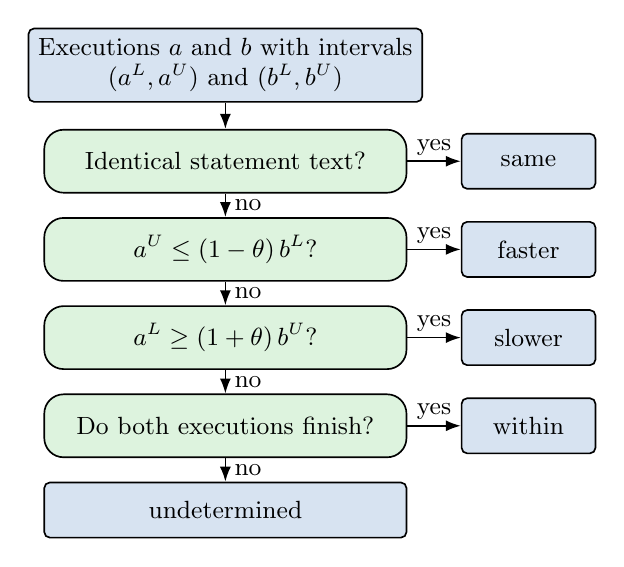
\begin{tikzpicture}[x=1cm,y=1cm]
  \node[store, minimum width=4.6cm] (in) at (0, 4.90) {Executions $a$ and $b$ with intervals\\$(a^{L}, a^{U})$ and $(b^{L}, b^{U})$};
  \node[dec, minimum width=4.6cm, minimum height=0.8cm] (d1) at (0, 3.68) {Identical statement text?};
  \node[dec, minimum width=4.6cm, minimum height=0.8cm] (d2) at (0, 2.56) {$a^{U} \le (1-\theta)\, b^{L}$?};
  \node[dec, minimum width=4.6cm, minimum height=0.8cm] (d3) at (0, 1.44) {$a^{L} \ge (1+\theta)\, b^{U}$?};
  \node[dec, minimum width=4.6cm, minimum height=0.8cm] (d4) at (0, 0.32) {Do both executions finish?};
  \node[store, minimum width=4.6cm] (o5) at (0, -0.75) {undetermined};

  \node[store, minimum width=1.7cm] (o1) at (3.85, 3.68) {same};
  \node[store, minimum width=1.7cm] (o2) at (3.85, 2.56) {faster};
  \node[store, minimum width=1.7cm] (o3) at (3.85, 1.44) {slower};
  \node[store, minimum width=1.7cm] (o4) at (3.85, 0.32) {within};

  \draw[flow] (in.south) -- (d1.north);
  \draw[flow] (d1.south) -- node[right, inner sep=3pt] {no} (d2.north);
  \draw[flow] (d2.south) -- node[right, inner sep=3pt] {no} (d3.north);
  \draw[flow] (d3.south) -- node[right, inner sep=3pt] {no} (d4.north);
  \draw[flow] (d4.south) -- node[right, inner sep=3pt] {no} (o5.north);
  \draw[flow] (d1.east) -- node[above, inner sep=2pt] {yes} (o1.west);
  \draw[flow] (d2.east) -- node[above, inner sep=2pt] {yes} (o2.west);
  \draw[flow] (d3.east) -- node[above, inner sep=2pt] {yes} (o3.west);
  \draw[flow] (d4.east) -- node[above, inner sep=2pt] {yes} (o4.west);
\end{tikzpicture}

  \caption{Outcome class of an execution $a$ against an execution $b$ according to~\eqref{eq:outcome}.}
  \label{fig:outcome}
\end{figure}
We call a statement \emph{improved} by an arm when the outcome of the arm against Original is \emph{faster}.
We call a comparison \emph{robust} when it holds under the end of each interval that is least favorable to it.

% ===========================================================================
\section{Results}
\label{sec:results}

The experiments proceed in layers: whether the layer helps where its pool is tuned (Section~\ref{sec:rq1}) and where it is not (Section~\ref{sec:rq2}), how the result changes with the data (Section~\ref{sec:rq3}), what the budget, the policy, and the sources contribute (Sections~\ref{sec:rq4} and~\ref{sec:rq5}), which evidence and cost stand behind the returned rewrites (Section~\ref{sec:rq6}), and whether the timings hold in a session with one cutoff (Section~\ref{sec:rq7}).

\begin{table}[t]
\caption{Mean and median latency in seconds, and outcomes against the original statement. Intervals follow~\eqref{eq:interval}. Rewr.: statements for which the arm returns a rewrite; F: faster; S: slower; U: undetermined.}
\label{tab:main}
\centering
\footnotesize
\setlength{\tabcolsep}{3.5pt}
\begin{tabular}{@{}lccrrrr@{}}
\toprule
Arm & Mean & Median & Rewr. & F & S & U \\
\midrule
\TabMainBody
\bottomrule
\end{tabular}
\end{table}

\begin{figure*}[t]
  \centering
  
\includegraphics{figures/plots/perquery_legend.pdf}\\[1pt]
  \subfloat[\textsc{Dev}, \DevN{} statements\label{fig:perquery-dev}]{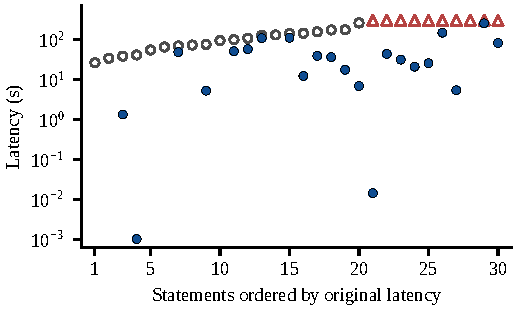
\includegraphics{figures/plots/perquery_dev.pdf}}\hfill
  \subfloat[Held-out, \HeldAllN{} statements\label{fig:perquery-held}]{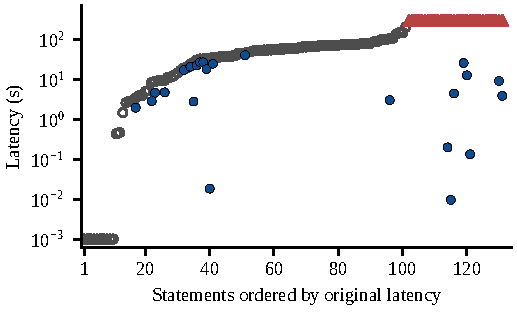
\includegraphics{figures/plots/perquery_heldAll.pdf}}
  \caption{Latency per statement: (a) development cohort; (b) held-out statements. Latencies below \SI{1}{\milli\second} are drawn at \SI{1}{\milli\second}.}
  \label{fig:perquery}
\end{figure*}

\subsection{Development Cohort}
\label{sec:rq1}

Table~\ref{tab:main} and Fig.~\ref{fig:perquery}\subref{fig:perquery-dev} show the result on \textsc{Dev}.
In Fig.~\ref{fig:perquery} a circle marks an original that finishes, a triangle an original that is cut off, and a filled dot the rewrite that \sys{} returns; a statement without a dot keeps its original.
\sys{} returns a rewrite for \DevOursRewrites{} of \DevN{} statements and all of them are improvements; mean latency falls from \secs{\DevOrigMean} to \secs{\DevOursMean}, a reduction of \pc{\DevOursRedU}.
The gain concentrates on statements that do not finish: \DevOrigCensored{} originals are cut off at \SI{\Tmax}{\second}, and \sys{} returns a finishing rewrite for \DevRescued{} of them.

Three facts bound what this cohort shows.
First, the pool is tuned on it. \DevSeededImproved{} of the \DevOursFaster{} improvements fall on the \SeededQueries{} statements with manually added hints, and \DevUnseededImproved{} fall on the other \DevUnseededN{} statements.
Second, none of its original timings is live. They come from earlier campaigns through the measurement cache, and timings drift between campaigns on this shared workstation: one TPC-H statement takes \secs{\DriftOld} in a run of one campaign and \secs{\DriftNew} in another.
Third, the earlier campaigns stop replayed rewrites early. \DevCutTwenty{} replayed rewrites are cut off, with a logged cutoff between \SI{20}{\second} and \SI{21}{\second} where the log records one, while cached timings of other candidates come from runs with cutoffs of up to \SI{\Tmax}{\second}.

The intervals make the third fact visible: the mean of R-Bot replay lies in \secs{\DevRbotMean}, and only its lower end is close to the \secs{\DevOursMean} of \sys{}.
In the paired view of Fig.~\ref{fig:paired}, \sys{} is faster than R-Bot replay on \DevRbotOursFaster{} statements and returns the same statement on \DevRbotOursSame{}; \DevRbotOursUndet{} comparisons are undetermined.
Against QUITE replay, whose mean lies in \secs{\DevQuiteMean}, \sys{} is robustly faster.

\begin{figure}[t]
  \centering
  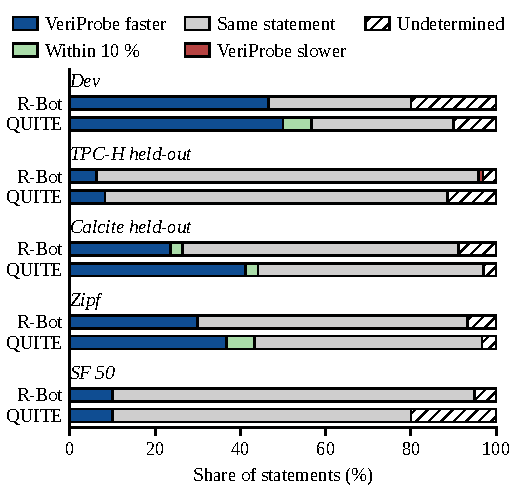
\includegraphics{figures/plots/paired.pdf}
  \caption{Outcome of \sys{} against each replay arm per cohort, as defined in~\eqref{eq:outcome}. Each bar covers all statements of the cohort.}
  \label{fig:paired}
\end{figure}

\subsection{Held-Out Statements}
\label{sec:rq2}

The held-out cohorts are the main test: their pool contains no manually added candidate, and \HeldAllOrigLive{} of their \HeldAllN{} originals are timed in the same campaign as their candidates.

\textbf{Against the original.}
\sys{} improves \HeldAllOursFaster{} of \HeldAllN{} statements (\pc{\HeldAllOursFasterPct}) and lowers mean latency from \secs{\HeldAllOrigMean} to \secs{\HeldAllOursMean} (\pc{\HeldAllOursRedU}).
On \textsc{Calcite} held-out, \CalciteHeldOursFaster{} of \CalciteHeldN{} statements improve and the mean falls by \pc{\CalciteHeldOursRedU}; these statements are written to trigger specific rewrite rules, and \CalciteHeldRescued{} originals that do not finish receive a finishing rewrite.
On \textsc{TPC-H} held-out, \TpchHeldOursFaster{} of \TpchHeldN{} statements improve and the mean falls by \pc{\TpchHeldOursRedU}.
For \TpchHeldOursSame{} TPC-H statements \sys{} returns the original, and Fig.~\ref{fig:perquery}\subref{fig:perquery-held} shows that the originals that are cut off stay cut off with few exceptions.
The pool explains this: the gate admits only \TpchHeldAccepted{} of \TpchHeldPool{} TPC-H candidates, and the probe cutoff of \SI{45}{\second} excludes every candidate that needs longer, although many originals run for more than \SI{60}{\second}.

\textbf{Against the replay arms.}
The logs decide few comparisons of a replayed rewrite with its original.
Of the \HeldAllQuiteRewrites{} QUITE rewrites that the gate admits, the logs show \HeldAllQuiteFaster{} faster than the original, \HeldAllQuiteSlower{} slower, and \HeldAllQuiteUndet{} undetermined; of the \HeldAllRbotRewrites{} admitted R-Bot rewrites they show \HeldAllRbotFaster{} faster, \HeldAllRbotSlower{} slower, and \HeldAllRbotUndet{} undetermined.
Most undetermined rewrites are never timed, because the arm reuses a probe that is cut off.
\sys{} is robustly faster than QUITE replay: its mean of \secs{\HeldAllOursMean} is below the lower end of \secs{\HeldAllQuiteMean}.

The comparison with R-Bot replay does not favor \sys{}.
The mean of R-Bot replay lies in \secs{\HeldAllRbotMean}, which contains the mean of \sys{}; on \textsc{TPC-H} held-out the replay is robustly better, \secs{\TpchHeldRbotMean} against \secs{\TpchHeldOursMean}.
One statement decides this in the logs.
Its original is cut off at \SI{\Tmax}{\second} and its replayed R-Bot rewrite takes \secs{\MissedReplay}.
This rewrite is in the pool of \sys{} and passes the gate, but \sys{} never probes it: two LLM proposals with lower planner cost use both probes, both are cut off, and \sys{} returns the original.
Section~\ref{sec:rq7} shows that this is not a single case.

\textbf{All cohorts.}
Fig.~\ref{fig:outcomes} extends the outcome columns of Table~\ref{tab:main} to all five cohorts: for every arm it shows the share of statements in each outcome class of~\eqref{eq:outcome}.
Only the replay arms have slower and undetermined shares; \sys{} has none because of its fallback.

\begin{figure*}[t]
  \centering
  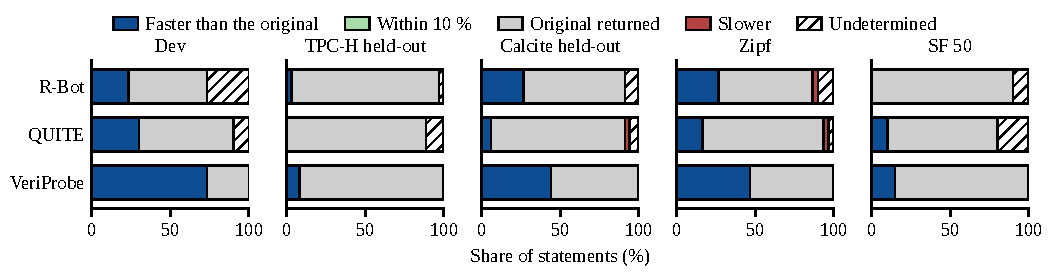
\includegraphics{figures/plots/outcomes.pdf}
  \caption{Outcome of each arm against the original statement per cohort, as defined in~\eqref{eq:outcome}.}
  \label{fig:outcomes}
\end{figure*}

\subsection{Skew and Scale}
\label{sec:rq3}

Fig.~\ref{fig:scaleskew} repeats two sets of statements on a second database.

\begin{figure}[t]
  \centering
  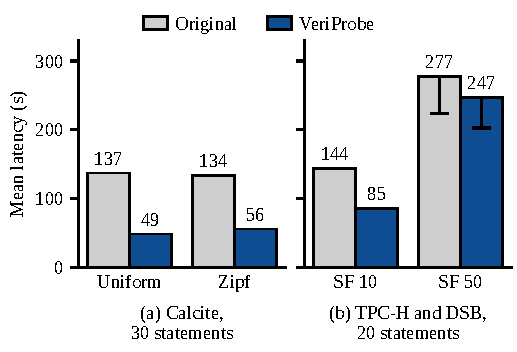
\includegraphics{figures/plots/skew_scale.pdf}
  \caption{Mean latency of the same statements on two databases: (a) uniform and Zipf data; (b) scale factors 10 and 50. A bar and the number above it show the upper end of~\eqref{eq:interval}; a whisker reaches down to the lower end where the two differ.}
  \label{fig:scaleskew}
\end{figure}

\textbf{Skew.}
On Zipf data all timings are live.
\sys{} improves \ZipfOursFaster{} of \ZipfN{} statements and lowers the mean from \secs{\ZipfOrigMean} to \secs{\ZipfOursMean} (\pc{\ZipfOursRedU}), close to the \pc{\UniformSameOursRedU} on the same statements with uniform data.
The improved statements overlap but are not identical: \SkewBothImproved{} improve on both databases, \SkewOnlyFirstImproved{} only on uniform data, and \SkewOnlySecondImproved{} only on Zipf data.
A rewrite that helps on one distribution is thus not a safe choice on another, which is the reason for selecting on the target database.
On this cohort \sys{} is robustly faster than both replay arms: their means lie in \secs{\ZipfRbotMean} and \secs{\ZipfQuiteMean}.

\textbf{Scale.}
At SF 50 the experiment is dominated by cutoffs: \ScaleOrigCensoredSecond{} of \SfFiftyN{} originals do not finish, against \ScaleOrigCensoredFirst{} at SF 10, and some are stopped after \SI{120}{\second}, so that even the mean of Original is an interval, \secs{\SfFiftyOrigMean}.
\sys{} improves \SfFiftyOursFaster{} statements, against \SfTenSameOursFaster{} of the same statements at SF 10, and its mean lies in \secs{\SfFiftyOursMean}.
The result is a statement about the time limits of our protocol more than about the rewrites, and we draw no conclusion on scalability from it.

\subsection{Budget}
\label{sec:rq4}

Fig.~\ref{fig:budget} varies the budget $M$ of the selection procedure.

\begin{figure}[t]
  \centering
  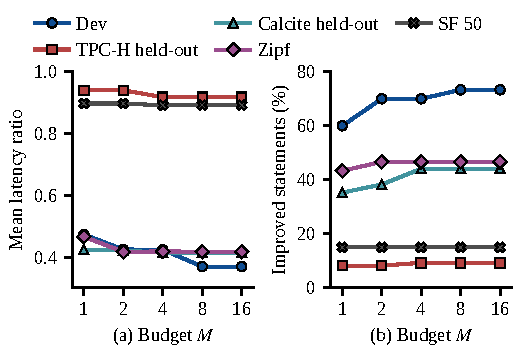
\includegraphics{figures/plots/budget.pdf}
  \caption{Effect of the budget $M$: (a) mean latency of \sys{} divided by that of Original, under the upper end of~\eqref{eq:interval}; (b) share of improved statements.}
  \label{fig:budget}
\end{figure}

A budget of one already yields most of the benefit: \DevBudgetOneImproved{} of the final \DevBudgetSixteenImproved{} improvements on \textsc{Dev} and \HeldAllBudgetOneImproved{} of \HeldAllBudgetSixteenImproved{} on the held-out statements.
The results do not change from $M = \DevBudgetSaturation$ on \textsc{Dev} and from $M = \HeldAllBudgetSaturation$ on the held-out statements.
The reason is the size of the admitted set: a held-out statement has \HeldAllAcceptedPerStatement{} admitted candidates on average, so a larger budget has nothing to explore.
The budget runs execute after the replay arms, whose full timings are in the cache and act as free probes; with $M = 16$ this yields \HeldAllBudgetSixteenImproved{} improved held-out statements, one more than the \HeldAllOursFaster{} of the first pass in Table~\ref{tab:main}.

\subsection{Policy Variants and Sources}
\label{sec:rq5}

Table~\ref{tab:variants} changes one element of the selection policy at a time on the same admitted candidates.
These variants are selections from the logged pool; they are not separate runs of the generators.

\begin{table}[t]
\caption{Selection policies on the same admitted candidates. Mean latency in seconds as in~\eqref{eq:mean}; F: faster than the original; S: slower; U: undetermined.}
\label{tab:variants}
\centering
\footnotesize
\setlength{\tabcolsep}{2.3pt}
\begin{tabular}{@{}>{\raggedright\arraybackslash}p{2.05cm}crrrcrrr@{}}
\toprule
 & \multicolumn{4}{c}{\textsc{Dev} (\DevN)} & \multicolumn{4}{c}{Held-out (\HeldAllN)} \\
\cmidrule(lr){2-5}\cmidrule(l){6-9}
Policy & Mean & F & S & U & Mean & F & S & U \\
\midrule
Full policy & \DevVarFullMean & \DevVarFullFaster & \DevVarFullSlower & \DevVarFullUndet & \HeldAllVarFullMean & \HeldAllVarFullFaster & \HeldAllVarFullSlower & \HeldAllVarFullUndet \\
Class A only & \DevVarClassAMean & \DevVarClassAFaster & \DevVarClassASlower & \DevVarClassAUndet & \HeldAllVarClassAMean & \HeldAllVarClassAFaster & \HeldAllVarClassASlower & \HeldAllVarClassAUndet \\
Class B only & \DevVarClassBMean & \DevVarClassBFaster & \DevVarClassBSlower & \DevVarClassBUndet & \HeldAllVarClassBMean & \HeldAllVarClassBFaster & \HeldAllVarClassBSlower & \HeldAllVarClassBUndet \\
No hint or join action & \DevVarNoSteerMean & \DevVarNoSteerFaster & \DevVarNoSteerSlower & \DevVarNoSteerUndet & \HeldAllVarNoSteerMean & \HeldAllVarNoSteerFaster & \HeldAllVarNoSteerSlower & \HeldAllVarNoSteerUndet \\
Generation order & \DevVarGenOrderMean & \DevVarGenOrderFaster & \DevVarGenOrderSlower & \DevVarGenOrderUndet & \HeldAllVarGenOrderMean & \HeldAllVarGenOrderFaster & \HeldAllVarGenOrderSlower & \HeldAllVarGenOrderUndet \\
Planner cost only & \DevVarCostOnlyMean & \DevVarCostOnlyFaster & \DevVarCostOnlySlower & \DevVarCostOnlyUndet & \HeldAllVarCostOnlyMean & \HeldAllVarCostOnlyFaster & \HeldAllVarCostOnlySlower & \HeldAllVarCostOnlyUndet \\
\bottomrule
\end{tabular}
\end{table}

\textbf{Probe and fallback.}
The last row removes steps 4 and 5: it returns the admitted candidate with the lowest planner cost.
On \textsc{Dev} this policy is robustly worse than the full policy, \secs{\DevVarCostOnlyMean} against \secs{\DevVarFullMean}.
On the held-out statements the logs decide little: \HeldAllVarCostOnlyFaster{} of its selections are faster than the original, \HeldAllVarCostOnlySlower{} are slower, and \HeldAllVarCostOnlyUndet{} are undetermined, because the campaign does not time them but reuses probes that are cut off.
Its mean lies in \secs{\HeldAllVarCostOnlyMean}, an interval that contains the means of Original and of the full policy.
The replay arms also select without probe and without fallback, and Section~\ref{sec:rq7} times their selections with one cutoff.

\textbf{Candidate classes.}
On \textsc{Dev}, class B candidates carry the result: class B alone reaches \secs{\DevVarClassBMean}, class A alone \secs{\DevVarClassAMean}.
On the held-out statements the picture reverses: class A alone reaches \secs{\HeldAllVarClassAMean}, which is \secs{\HeldAllClassAGap} above the full policy, and class B alone reaches \secs{\HeldAllVarClassBMean}.
Fig.~\ref{fig:sources} shows the same reversal per source.
The class B candidates that matter on \textsc{Dev} are the ones that we add there; the frozen LLM proposals alone produce \HeldAllSrcMacro{} of the \HeldAllOursFaster{} held-out improvements.
The honest reading is that the gain of \sys{} on unseen statements comes mostly from selecting rule rewrites safely, and that LLM proposals add a smaller part.

\textbf{Priority order and planner hints.}
Replacing the order of~\eqref{eq:priority} by the order of generation costs \secs{\DevGenOrderLoss} of mean latency on \textsc{Dev}; on the held-out statements the mean stays in \secs{\HeldAllVarGenOrderMean}, with one run cut off.
The order decides which candidates are probed, so it matters only when pools are deep.
The fourth row removes every candidate that contains a planner hint or whose action targets a join or a materialization, and it uses the order of generation.
The mean on \textsc{Dev} rises to \secs{\DevVarNoSteerMean}, and \DevSrcHint{} of the improvements on \textsc{Dev} are hints on the unchanged statement text.
These hints belong to the manually tuned part of the pool; no held-out improvement uses a hint.

\begin{figure}[t]
  \centering
  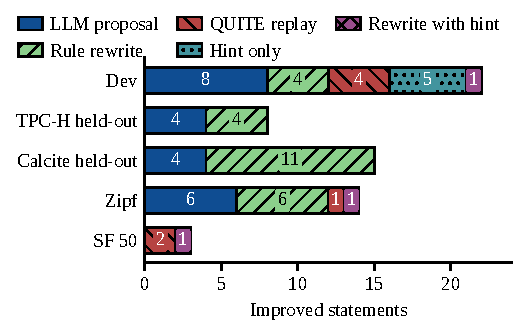
\includegraphics{figures/plots/sources.pdf}
  \caption{Source of the rewrite that \sys{} returns for each improved statement; the numbers are statement counts. A rule rewrite is the output of Calcite rules, including replayed R-Bot rewrites; a hint only candidate keeps the original text.}
  \label{fig:sources}
\end{figure}

\subsection{Evidence and Cost of Selection}
\label{sec:rq6}

\textbf{Evidence.}
Over all \AllPairs{} pairs of database and statement, \sys{} returns \AllSelected{} rewrites.
\AllEvSyntactic{} carry the label \emph{syntactic}, \AllEvStructural{} the label \emph{formal} through the structural check, and \AllEvDifferential{} the label \emph{bounded}.
SQLSolver contributes no admitted candidate in these campaigns. The gate passes only a narrow fragment to it and allows it one second per pair, and the log does not separate these two causes.
Only \pc{\AllEvFormalPct} of the selected rewrites are thus backed by evidence for all instances.
All \HeldAllOursFaster{} held-out improvements are \emph{bounded}.
The gate is selective: it rejects \pc{\AllRejectedPct} of the \AllPool{} candidates, and \pc{\TpchHeldRejectedPct} on \textsc{TPC-H} held-out.
Fig.~\ref{fig:funnel} shows this funnel per cohort; the campaign log stores admitted candidates only, so we cannot break the rejections down by reason.
For the DBA of our scenario, a \emph{bounded} rewrite is a suggestion that has survived six test databases, not a proven replacement.

\begin{figure}[t]
  \centering
  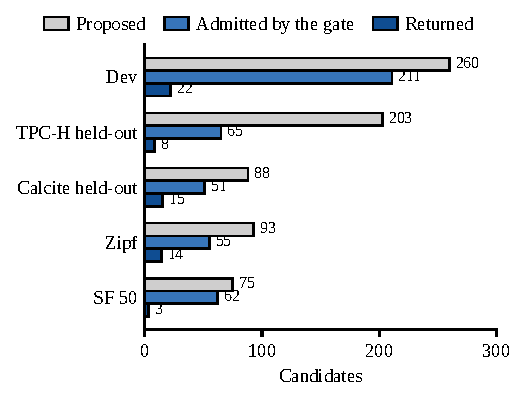
\includegraphics{figures/plots/funnel.pdf}
  \caption{Candidates per cohort: proposed by the sources, admitted by the gate, and returned by \sys{}.}
  \label{fig:funnel}
\end{figure}

\textbf{Cost.}
We bound the executions that selection adds by~\eqref{eq:cost} and relate them to the saving per execution by~\eqref{eq:amortize}, counting an original that is cut off at its cutoff.
For the \BreakevenN{} improved pairs the median of $n(q)$ is \BreakevenMedian{} executions and the 90th percentile is \BreakevenPninety{}; \BreakevenWithinFive{} pairs recover the cost within five executions, and the largest value is \BreakevenMax{}.
Fig.~\ref{fig:breakeven} shows the full distribution.

\begin{figure}[t]
  \centering
  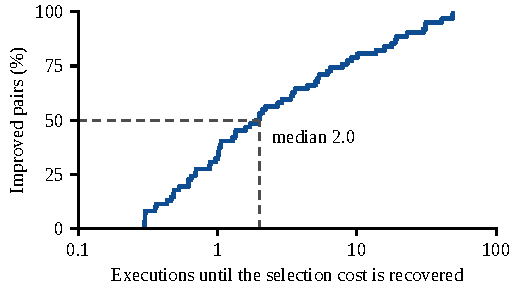
\includegraphics{figures/plots/breakeven.pdf}
  \caption{Cumulative share of improved pairs over $n(q)$ of~\eqref{eq:amortize}, the number of executions after which the saving covers the cost bound of~\eqref{eq:cost}.}
  \label{fig:breakeven}
\end{figure}

For the statements that \sys{} does not improve, the cost is spent without return; on \textsc{TPC-H} held-out this is the common case.
The bound excludes the gate, whose runs on the small databases the campaign does not time.

\subsection{Validation Session with Equal Cutoffs}
\label{sec:rq7}

The campaigns leave two doubts open: the arms run with different cutoffs, and \sys{} selects on the runs that we report.
A separate session addresses both.

\textbf{Protocol.}
For each pair of database and statement for which at least one arm returns a rewrite, the session times the original and every returned rewrite with the same cutoff $T_{\max}$.
It runs three rounds (Fig.~\ref{fig:protocol}). Each round executes every statement of the pair once, and the order rotates by one position per round, so that load on the host affects all statements of a pair alike.
A statement that reaches the cutoff does not run again.
The latency of a statement is the median of its three rounds, where a round that is cut off counts as at least $T_{\max}$; a statement that is cut off in its first round has no other round and is reported as cut off.
The session selects nothing.
It covers \ValCoverageLong{}, and Table~\ref{tab:validation} lists the covered pairs per cohort.

\begin{table*}[t]
\caption{Validation session with one cutoff for all statements. Mean: mean latency in seconds over the covered pairs, where an arm without a rewrite counts with the original and an interval arises when a statement is cut off after a round that finishes. Rewr.: rewrites timed; F: faster than the original; W: within \SI{\ThetaPct}{\percent}; S: slower; U: undetermined.}
\label{tab:validation}
\centering
\footnotesize
\setlength{\tabcolsep}{2.7pt}
\begin{tabular}{@{}llc crrrrr crrrrr crrrrr@{}}
\toprule
 & & & \multicolumn{6}{c}{R-Bot replay} & \multicolumn{6}{c}{QUITE replay} & \multicolumn{6}{c}{\sys{}} \\
\cmidrule(lr){4-9}\cmidrule(lr){10-15}\cmidrule(l){16-21}
Cohort & Pairs & Original & Mean & Rewr. & F & W & S & U & Mean & Rewr. & F & W & S & U & Mean & Rewr. & F & W & S & U \\
\midrule
\TabValBody
\bottomrule
\end{tabular}
\end{table*}

\begin{figure}[t]
  \centering
  % Order of the runs in the validation session for one pair of database and statement.
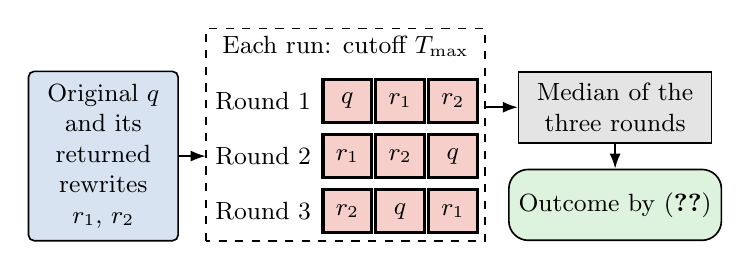
\begin{tikzpicture}[x=1cm,y=1cm]
  \node[store, minimum width=1.90cm, minimum height=2.15cm] (in) at (0.95, 1.00) {Original $q$\\and its\\returned\\rewrites\\$r_1$, $r_2$};

  \draw[dashed, line width=0.6pt] (2.25, -0.08) rectangle (5.80, 2.62);
  \node[anchor=north, inner sep=2pt] at (4.025, 2.60) {Each run: cutoff $T_{\max}$};
  \foreach \k/\y/\a/\b/\c in {1/1.70/q/r_1/r_2, 2/1.00/r_1/r_2/q, 3/0.30/r_2/q/r_1} {
    \node[anchor=west, inner sep=1pt] at (2.33, \y) {Round \k};
    \node[exec, minimum width=0.62cm, minimum height=0.55cm, inner sep=0pt] at (4.05, \y) {$\a$};
    \node[exec, minimum width=0.62cm, minimum height=0.55cm, inner sep=0pt] at (4.72, \y) {$\b$};
    \node[exec, minimum width=0.62cm, minimum height=0.55cm, inner sep=0pt] at (5.39, \y) {$\c$};
  }

  \node[proc, minimum width=2.45cm, minimum height=0.9cm] (med) at (7.45, 1.62) {Median of the\\three rounds};
  \node[dec, minimum width=2.45cm, minimum height=0.9cm] (out) at (7.45, 0.38) {Outcome by \eqref{eq:outcome}};

  \draw[flow] (in.east) -- (2.25, 1.00);
  \draw[flow] (5.80, 1.62) -- (med.west);
  \draw[flow] (med.south) -- (out.north);
\end{tikzpicture}

  \caption{Order of the runs in the validation session for a pair with two returned rewrites. Steps with a heavy outline execute on the target database.}
  \label{fig:protocol}
\end{figure}

\begin{figure}[t]
  \centering
  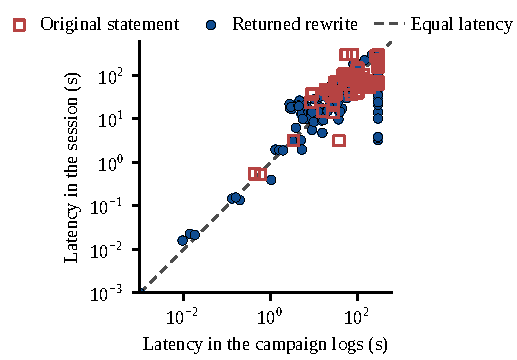
\includegraphics{figures/plots/validation_scatter.pdf}
  \caption{Latency of each statement in the validation session against its latency in the campaign logs. A run that is cut off is drawn at $T_{\max}$.}
  \label{fig:valscatter}
\end{figure}

\textbf{Noise.}
Other jobs load the workstation during the session.
The slowest of the three rounds of a statement takes \ValSpreadMedian{} times as long as the fastest at the median and \ValSpreadPninety{} times at the 90th percentile.
This spread exceeds the tolerance $\theta$, so a verdict close to the tolerance is not reliable.
We call a verdict \emph{separated} when all three rounds of the faster statement finish and each of them is shorter than every round of the other statement, where a round that is cut off counts as $T_{\max}$.

\textbf{Returned rewrites.}
The session times \ValOursTimed{} rewrites that \sys{} returns in the campaigns.
It finds \ValOursConfirmed{} of them again faster than the original (\ValAllOursFasterSep{} separated), \ValOursNotConfirmedWithin{} within \SI{\ThetaPct}{\percent} of the original, \ValOursNotConfirmedSlower{} slower, and \ValOursNotConfirmedUndet{} undetermined.

\textbf{Replay arms.}
On the covered pairs the campaign logs leave \ValReplayUndetTimed{} comparisons of a replayed rewrite with its original undetermined.
With one cutoff, the session finds \ValReplayUndetNowFaster{} of these rewrites faster than the original, \ValReplayUndetNowWithin{} within \SI{\ThetaPct}{\percent}, \ValReplayUndetNowSlower{} slower, and \ValReplayUndetStill{} still undetermined.
On the held-out pairs it finds \ValHeldAllRbotFaster{} of the \ValHeldAllRbotRewrites{} R-Bot rewrites faster than the original (\ValHeldAllRbotFasterSep{} separated) and \ValHeldAllRbotSlower{} slower (\ValHeldAllRbotSlowerSep{} separated); of the \ValHeldAllQuiteRewrites{} QUITE rewrites it finds \ValHeldAllQuiteFaster{} faster (\ValHeldAllQuiteFasterSep{} separated) and \ValHeldAllQuiteSlower{} slower (\ValHeldAllQuiteSlowerSep{} separated).

\textbf{Probing against planner cost.}
On the \ValHeldAllDone{} held-out pairs the two selection principles miss different statements.
On \ValHeldAllMissedOrigCutOff{} pairs \sys{} keeps an original that is cut off, although a replayed rewrite finishes, in \secs{\ValHeldAllMissedMin} to \secs{\ValHeldAllMissedMax}.
Each of these rewrites is in the pool of \sys{} and passes the gate.
In the campaign, \sys{} probes \ValHeldAllRescueProbed{} of them and the probe is cut off, \ValHeldAllRescueInherited{} inherits the cut off probe of a candidate with the same estimated plan, and \ValHeldAllRescueNotProbed{} is never probed, because candidates with lower planner cost use both probes.
In the session, \ValHeldAllMissedOverCap{} of the rewrites take longer than the probe cap of \SI{\ProbeCap}{\second} and \ValHeldAllMissedUnderCap{} finish below it, so the cap alone does not explain the loss; a probe is a single run without warmup, and the log does not record how long a probe runs before it is cut off.
Conversely, on \ValHeldAllOursOnly{} pairs \sys{} returns a faster rewrite while neither replay arm does: \ValHeldAllOursOnlyRule{} of these rewrites are rule rewrites that the cost filter of R-Bot replay rejects, and \ValHeldAllOursOnlyMacro{} are LLM proposals.
The first effect dominates the mean, because it concerns originals that do not finish: the mean latency on these pairs is \secs{\ValHeldAllOrigMean} for Original, \secs{\ValHeldAllRbotMean} for R-Bot replay, \secs{\ValHeldAllQuiteMean} for QUITE replay, and \secs{\ValHeldAllOursMean} for \sys{}.
Keeping the fastest timed statement of each pair gives \secs{\ValHeldAllBestMean}.
On the held-out statements R-Bot replay therefore outperforms \sys{}, and the probe step is the cause.

\textbf{Timing level.}
Absolute latencies differ between the session and the campaign logs, and the direction depends on the cohort (Fig.~\ref{fig:valscatter}).
For the \ValDevDriftN{} covered originals of \textsc{Dev} that finish in both, the latency in the session is \ValDevDriftMin{} to \ValDevDriftMax{} times the latency in the logs, with a median factor of \ValDevDriftMedian{}.
For the \ValHeldAllDriftN{} held-out originals the factor is \ValHeldAllDriftMin{} to \ValHeldAllDriftMax{}, with a median of \ValHeldAllDriftMedian{}.
The session finishes \ValOrigNowFinished{} of the \ValOrigCampaignCutOff{} covered originals that the logs record as cut off, and it cuts off \ValOrigNowCutOff{} of the \ValOrigCampaignFinished{} that finish in the logs.
A latency in this paper therefore holds for the session that measures it, and we compare statements only within one session.

% ===========================================================================
\section{Limitations and Threats to Validity}
\label{sec:limits}

\textbf{Replays are not the baselines themselves.}
The replay arms apply published rewrites on our server and under our gate.
A fresh run of either system can produce other rewrites, so our results describe the published rewrites, not the systems.

\textbf{Selection and report use the same runs.}
The fallback compares the three timed runs that we also report.
That no selected rewrite is slower in the campaigns is therefore a property of~\eqref{eq:decision} and not an empirical finding, and the reported latency of a selected rewrite is slightly optimistic.
The validation session of Section~\ref{sec:rq7} removes this dependence for \ValCoverageShort{}.

\textbf{The development cohort is assembled.}
Its timings come from several campaigns and its pool is tuned on it (Section~\ref{sec:rq1}).
On the \ValDevDone{} of its pairs that the validation session covers, the mean latency of the original is \secs{\ValDevOrigMean} in the session against \secs{\ValDevCampaignOrigMean} in the logs.
No claim of this paper rests on this cohort alone.

\textbf{Bounded evidence.}
\AllEvDifferential{} of \AllSelected{} selected rewrites are not proven equivalent.
The gate never compares results on the target database.

\textbf{Server and time limits.}
The server has little memory and no parallelism, so originals are slow and \HeldAllOrigCensored{} of \HeldAllN{} held-out originals do not finish.
On a tuned server fewer statements leave room for improvement.
The probe is the weakest step of the layer: it is a single run without warmup under a fixed cap, and it rejects rewrites that finish while their originals do not (Section~\ref{sec:rq7}).
A probe cutoff equal to that of the original removes this loss at the price of longer probes; we do not evaluate it.

\textbf{Coverage.}
We evaluate 10 of 232 DSB statements; no campaign covers the other 222.
The campaign on the 58 Calcite statements of QUITE stops on a schema file that the gate cannot match to the database catalog.
The held-out result covers TPC-H and Calcite only.

\textbf{No search, one model.}
The priority order is a fixed heuristic, and the LLM candidates are frozen proposals of one model from one generation pass; another model, or repeated sampling, changes the pool.
The code base contains a Monte Carlo tree search controller~\cite{kocsis2006} that generates candidates during search; we do not evaluate it, and none of our results speaks about tree search.

% ===========================================================================
\section{Related Work}
\label{sec:related}

\textbf{Rule-based rewriting.}
Rule sets inside optimizers date back to Starburst and Cascades~\cite{pirahesh1992,graefe1995}, and Calcite makes a large rule set reusable~\cite{begoli2018}.
A learned system explores the order of rule application with Monte Carlo tree search~\cite{zhou2021}; WeTune discovers and verifies new rules~\cite{wang2022}, SlabCity synthesizes whole statements~\cite{dong2023}, and QueryBooster lets users supply rules~\cite{bai2023}.
\sys{} consumes the output of such systems as class A candidates.

\textbf{LLM-based rewriting.}
LLM-R2 lets an LLM recommend Calcite rules~\cite{li2024}, R-Bot adds retrieved evidence and stepwise reflection~\cite{sun2025}, and GenRewrite and QUITE let the model write the statement~\cite{liu2026,song2025}.
Closest to our work, the tool of Lee et al.\ for Microsoft SQL Server~\cite{lee2026} and ReSequel~\cite{fathollahzadeh2026} combine LLM rewriting with verification and execution, each for its own generator.
\sys{} is a layer over several generators, including the published output of other systems; it anchors every decision on the original statement, labels the evidence of what it returns, and reports results as intervals.
We make no claim that its verification is stronger than theirs.

\textbf{Equivalence checking.}
Provers for SQL equivalence include Cosette~\cite{chu2017}, EQUITAS~\cite{zhou2019}, SPES~\cite{zhou2022}, SQLSolver~\cite{ding2023}, and QED~\cite{wang2024}; VeriEQL checks equivalence up to a bound~\cite{he2024}.
The gate uses SQLSolver for a fragment and bounded testing otherwise; SQLSolver contributes no admitted candidate in our campaigns (Section~\ref{sec:rq6}), which is a limit of our integration.

% ===========================================================================
\section{Conclusion}
\label{sec:conclusion}

For recurring analytical statements on PostgreSQL we place one selection layer on top of several rewrite generators.
The layer admits a candidate only through an equivalence gate, probes at most two candidates on the target database, and falls back to the original statement.
On \HeldAllN{} held-out statements it improves \HeldAllOursFaster{} and lowers mean latency by \pc{\HeldAllOursRedU}, and a session with one cutoff finds \ValHeldAllOursFaster{} of \ValHeldAllOursRewrites{} returned rewrites faster again.
The layer is better than a replay of published QUITE rewrites.
It is not better than a replay of published R-Bot rewrites: its single capped probe rejects rewrites that finish while their originals do not, although it also finds rewrites that the planner cost rejects.
Most of its selected rewrites rest on bounded testing.
Three steps follow directly from these limits: a probe cutoff equal to that of the original, provers with wider coverage, and fresh runs of the compared systems.
Reporting cut off runs as intervals, and timing all arms again with one cutoff, are independent of our system; we recommend both for any comparison of rewriters whose time limits differ.

\label{lastcontent}% end of the pages that count towards the 12-page limit

\section*{Acknowledgment}
\emph{Disclosure of content generated by artificial intelligence (AI).}
The candidate rewrites that Section~\ref{sec:sources} calls LLM proposals are generated by the model gpt-6.1-sol.
The text of Sections~\ref{sec:intro} to~\ref{sec:conclusion}, all figures and tables, and the analysis and plotting scripts behind them are drafted with AI coding assistants (Claude and Gemini, used through the Cursor editor) from the campaign logs and reviewed by the author.
The experiment code is developed with AI coding assistants.

% ===========================================================================
\begin{thebibliography}{26}

\bibitem{pirahesh1992}
H.~Pirahesh, J.~M. Hellerstein, and W.~Hasan, ``Extensible/rule based query rewrite optimization in Starburst,'' in \emph{Proc. ACM SIGMOD Int. Conf. Manage. Data}, 1992, pp. 39--48.

\bibitem{graefe1995}
G.~Graefe, ``The Cascades framework for query optimization,'' \emph{IEEE Data Eng. Bull.}, vol.~18, no.~3, pp. 19--29, 1995.

\bibitem{chaudhuri1998}
S.~Chaudhuri, ``An overview of query optimization in relational systems,'' in \emph{Proc. ACM SIGACT-SIGMOD-SIGART Symp. Princ. Database Syst.}, 1998, pp. 34--43.

\bibitem{begoli2018}
E.~Begoli, J.~Camacho-Rodr\'iguez, J.~Hyde, M.~J. Mior, and D.~Lemire, ``Apache Calcite: A foundational framework for optimized query processing over heterogeneous data sources,'' in \emph{Proc. ACM SIGMOD Int. Conf. Manage. Data}, 2018, pp. 221--230.

\bibitem{zhou2021}
X.~Zhou, G.~Li, C.~Chai, and J.~Feng, ``A learned query rewrite system using Monte Carlo tree search,'' \emph{Proc. VLDB Endow.}, vol.~15, no.~1, pp. 46--58, 2021.

\bibitem{li2024}
Z.~Li, H.~Yuan, H.~Wang, G.~Cong, and L.~Bing, ``LLM-R2: A large language model enhanced rule-based rewrite system for boosting query efficiency,'' \emph{Proc. VLDB Endow.}, vol.~18, no.~1, pp. 53--65, 2024.

\bibitem{sun2025}
Z.~Sun, X.~Zhou, G.~Li, X.~Yu, J.~Feng, and Y.~Zhang, ``R-Bot: An LLM-based query rewrite system,'' \emph{Proc. VLDB Endow.}, vol.~18, no.~12, pp. 5031--5044, 2025.

\bibitem{liu2026}
J.~Liu and B.~Mozafari, ``GenRewrite: Query rewriting via large language models,'' \emph{Proc. ACM Manag. Data}, vol.~4, no.~1, pp. 1--26, 2026.

\bibitem{song2025}
Y.~Song, H.~Yan, J.~Lao, Y.~Wang, Y.~Li, Y.~Zhou, J.~Wang, and M.~Tang, ``QUITE: A query rewrite system beyond rules with LLM agents,'' arXiv:2506.07675, 2025.

\bibitem{leis2015}
V.~Leis, A.~Gubichev, A.~Mirchev, P.~Boncz, A.~Kemper, and T.~Neumann, ``How good are query optimizers, really?'' \emph{Proc. VLDB Endow.}, vol.~9, no.~3, pp. 204--215, 2015.

\bibitem{lee2026}
K.~Lee, A.~Dutt, V.~Narasayya, and S.~Chaudhuri, ``Verified LLM-based query rewriting for Microsoft SQL Server,'' \emph{Proc. VLDB Endow.}, vol.~19, no.~12, pp. 4594--4597, 2026.

\bibitem{fathollahzadeh2026}
S.~Fathollahzadeh, E.~Mansour, and M.~Boehm, ``ReSequel: Robust LLM-assisted query rewriting and optimization using templatization and sampling,'' \emph{Proc. VLDB Endow.}, vol.~19, no.~10, pp. 2880--2893, 2026.

\bibitem{chu2017}
S.~Chu, C.~Wang, K.~Weitz, and A.~Cheung, ``Cosette: An automated prover for SQL,'' in \emph{Proc. Conf. Innov. Data Syst. Res.}, 2017.

\bibitem{zhou2019}
Q.~Zhou, J.~Arulraj, S.~B. Navathe, W.~Harris, and D.~Xu, ``Automated verification of query equivalence using satisfiability modulo theories,'' \emph{Proc. VLDB Endow.}, vol.~12, no.~11, pp. 1276--1288, 2019.

\bibitem{zhou2022}
Q.~Zhou, J.~Arulraj, S.~B. Navathe, W.~Harris, and J.~Wu, ``SPES: A symbolic approach to proving query equivalence under bag semantics,'' in \emph{Proc. IEEE Int. Conf. Data Eng.}, 2022, pp. 2735--2748.

\bibitem{ding2023}
H.~Ding, Z.~Wang, Y.~Yang, D.~Zhang, Z.~Xu, H.~Chen, R.~Piskac, and J.~Li, ``Proving query equivalence using linear integer arithmetic,'' \emph{Proc. ACM Manag. Data}, vol.~1, no.~4, pp. 227:1--227:26, 2023.

\bibitem{wang2024}
S.~Wang, S.~Pan, and A.~Cheung, ``QED: A powerful query equivalence decider for SQL,'' \emph{Proc. VLDB Endow.}, vol.~17, no.~11, pp. 3602--3614, 2024.

\bibitem{he2024}
Y.~He, P.~Zhao, X.~Wang, and Y.~Wang, ``VeriEQL: Bounded equivalence verification for complex SQL queries with integrity constraints,'' \emph{Proc. ACM Program. Lang.}, vol.~8, no. OOPSLA1, pp. 1071--1099, 2024.

\bibitem{pghintplan}
Nippon Telegraph and Telephone Corporation, ``pg\_hint\_plan,'' release REL14\_1\_4\_3. [Online]. Available: https://github.com/ossc-db/pg\_hint\_plan

\bibitem{marcus2021}
R.~Marcus, P.~Negi, H.~Mao, N.~Tatbul, M.~Alizadeh, and T.~Kraska, ``Bao: Making learned query optimization practical,'' in \emph{Proc. ACM SIGMOD Int. Conf. Manage. Data}, 2021, pp. 1275--1288.

\bibitem{tpch}
Transaction Processing Performance Council, ``TPC Benchmark H (decision support) standard specification, revision 3.0.1.'' [Online]. Available: https://www.tpc.org/tpch/

\bibitem{ding2021}
B.~Ding, S.~Chaudhuri, J.~Gehrke, and V.~Narasayya, ``DSB: A decision support benchmark for workload-driven and traditional database systems,'' \emph{Proc. VLDB Endow.}, vol.~14, no.~13, pp. 3376--3388, 2021.

\bibitem{dong2023}
R.~Dong, J.~Liu, Y.~Zhu, C.~Yan, B.~Mozafari, and X.~Wang, ``SlabCity: Whole-query optimization using program synthesis,'' \emph{Proc. VLDB Endow.}, vol.~16, no.~11, pp. 3151--3164, 2023.

\bibitem{kocsis2006}
L.~Kocsis and C.~Szepesv\'ari, ``Bandit based Monte-Carlo planning,'' in \emph{Proc. Eur. Conf. Mach. Learn.}, 2006, pp. 282--293.

\bibitem{wang2022}
Z.~Wang, Z.~Zhou, Y.~Yang, H.~Ding, G.~Hu, D.~Ding, C.~Tang, H.~Chen, and J.~Li, ``WeTune: Automatic discovery and verification of query rewrite rules,'' in \emph{Proc. ACM SIGMOD Int. Conf. Manage. Data}, 2022, pp. 94--107.

\bibitem{bai2023}
Q.~Bai, S.~Alsudais, and C.~Li, ``QueryBooster: Improving SQL performance using middleware services for human-centered query rewriting,'' \emph{Proc. VLDB Endow.}, vol.~16, no.~11, pp. 2911--2924, 2023.

\end{thebibliography}

\end{document}
